\documentclass[12pt, letterpaper, fleqn]{report}

%\usepackage{hyperref}
\usepackage[pdftex]{graphicx}
\usepackage{color}
% usepackage{floatflt}
\usepackage{fancyhdr}
\usepackage{amsmath, epsfig}
\usepackage{url}
\usepackage{algorithmic}
\usepackage{algorithm}
\usepackage{pdfpages}
\numberwithin{algorithm}{chapter}
% \usepackage{spconf, amsmath, epsfig}
\usepackage{geometry}
%\usepackage[pdftex]{hyperref}
\geometry{verbose, letterpaper, dvips,
		  lmargin=1.5in, rmargin=1.0in,
		  tmargin=1.0in, bmargin=1.25in,
		  head=12pt, nofoot}

%--- This package contains local macros.  Remove the "draft" option (or
%--- (or change it to "final") for the final version --------
\usepackage[final]{thesisMacros}

\PageHeaders

\begin{document}

  \setcounter{page}{0}
  \pagenumbering{roman}

  \topskip=0pt
  \baselineskip=13pt
  \parskip=10pt % for toc
  \parindent 3mm

  \setcounter{page}{0}
\thispagestyle{empty}

\begin{center}
University of Nevada\\
Reno

\vfill


{\Large \bf An Extensible Component-based Approach to Simulation Systems on Heterogeneous Clusters\\ \vspace{0.05in}}
\vfill

A dissertation submitted in partial fulfillment of the\\
requirements for the degree of Doctor of Philosophy\\
in Computer Science

\vfill

by

\vspace{0.5in}

Roger Viet Hoang

\vspace{0.5in}

Dr. Frederick C. Harris, Jr., Dissertation Advisor

\vspace{0.5in}

May, 2014
\end{center}


  \BodySpacing

% \input{signaturePage.tex}
\thispagestyle{empty}
\pagenumbering{gobble}
%\includepdf[pages={1}]{figures/committee.pdf}
  \setcounter{page}{1}
  \pagenumbering{roman}

  % table of contents:
  % the .toc file generated isn't entirely accurate. If you run latex & bibtex a few times
  % so it generates everything, and look at the table of contents, it will show the list
  % of figures and list of rables page numbers to be on less than the actually are. To hack
  % a fix for it (assuming of course that it's really latex's fault and not mine), you can
  % open the .toc file and edit the numbers that will be displayed in the table of contents.
  % Then, run latex once. This will change the table of contents to the numbers you edited
  % in the .toc file. But running latex again will overwrite your changes.
    \newpage
\addcontentsline{toc}{chapter}{Abstract}
\begin{center}
  {\bf Abstract}
\end{center}

There is an abundance of computing power sitting in computer labs waiting
to be harnessed. Previous research in this area has shown promising results
networking clusters of workstations together in order to solve bigger problems
faster at a fraction of the cost for supercomputer time. There are, of course,
challenges to using these sorts of clusters: the communication fabrics linking
these machines aren't necessarily high-performance, and the differences
between individual machines in the cluster require careful load balancing in
order to efficiently use them. These problems have only become greater with
the introduction of acceleration hardware such as GPUs and FPGAs; however, that
hardware also provides even greater computing power at an even lower price
point for those that can work around their idiosyncracies. This dissertation
presents an approach to designing software to effectively utilize these heterogeneous
computing clusters in a modular, extensible manner. We apply it to the development
of a large-scale Neo-Cortical Simulator(NCS) as well as the engineering of a
virtual reality library, caVR.

    \newpage
\addcontentsline{toc}{chapter}{Dedication}
\begin{center}
\textbf{Dedication}

\vspace{0.2in}
For Allison. Yeah buddy.
\end{center}

    \newpage
\addcontentsline{toc}{chapter}{Acknowledgments}
\begin{center}
  \bf {Acknowledgments}
\end{center}

Something something about grants. Something something, long hashed grant numbers.
Maybe something inspirational. Thanking some committee people. Friends, colleagues, etc.
Don't think twice, it's alright.

  {

    \TOCSpacing

    \tableofcontents

    \newpage
    %\phantomsection\label{fsdjkaflsdjfl}
    \addcontentsline{toc}{chapter}{List of Tables}
    \listoftables

    \newpage
    %\phantomsection\label{sdjafklsdjfal}
    \addcontentsline{toc}{chapter}{List of Figures}
    \listoffigures

	% \nocite{*} % This line affects the bibliography.  If it is uncommented, then
				 % entries in the bibliography that aren't actually referenced in the
				 % paper will still be placed in the bibliography. Without this line,
				 % entries may still be placed in the .bib file, but the entries that
				 % are not used throughout the paper are no added to the created
				 % bibliography pages.
  }

  % actual text
  {
	\newpage
	\setcounter{page}{0}
	\pagenumbering{arabic}

	\BodySpacing

	\chapter{Introduction}
\label{chapter:intro}

Experiments in the field of neuroscience have traditionally been conducted using invasive physical methods including \emph{in vivo} (using a living organism) and \emph{in vitro} (in an artificial laboratory environment) methods. These methods, while effective in small-scale experiments, become impractical for performing experiments on a larger scale and are often times quite expensive. To combat these problems, neuroscientists have turned to \emph{in silico} methods to perform experiments, a field known as computational neuroscience. To create neurological experiments in a computer environment, a number of neural simulators that allow researchers to model biologically realistic neurons and neural networks have been created\cite{sejnowski1988computational}. These neural simulators allow researchers to build, run, and output the results of a simulation. While each simulator has the same goal in mind, they each have a different set of features and limitations. Researchers must choose which simulator provides the most appropriate set of functionality for their experiments \cite{brette2007simulation}.

The University of Nevada has created its own neural simulator called NCS, or Neo-Cortical Simulator. NCS tends to focus on larger scale simulations that involve large numbers of neurons and synapses. Performance was also a key consideration when designing NCS, and as a result the simulator was designed to be as fast as possible without adding features that would create additional computational overhead. By ensuring that the simulator is as fast as possible, NCS can run a million-cell model in realtime \cite{hoang2013novel}.

Although very fast and scalable, the NCS simulator by itself does not provide a convenient way for researchers to perform common tasks surrounding the simulation in an intuitive way. NCS provides a thin and feature-limited Python layer that allows it to be used with Python-based programs. This thin layer exposes the minimal features that NCS provides, such as adding neurons and synapses to the simulation. To make the NCS simulator a more useful tool for neuroscientists, additional higher-level features must be added that augment the minimalist approach to designing NCS. These features should provide neuroscientists the ability to easily create models, configure simulations, manage the data generated by simulations, and visualize their results. 

To accomplish this task, we have created a suite of tools that surround the NCS simulator in the form of a web-based interface and higher-level Python interface that gives a much more intuitive medium for interacting with the brain simulator. The web-based interface provides the ability for neuroscientists to create simulations without programming experience, and the Python interface provides high-level access using an easy-to-use Python library. This thesis covers the development and implementation of these tools, as well as the architectural and design choices that were made when creating them. The rest of this thesis is formatted as follows: Chapter 2 discusses background topics surrounding these tools; Chapter 3 details the design and implementation of the software; Chapter 4 presents conclusions and discusses possible future work that could be implemented in the software.
  \chapter{Background}
\label{chapter:background}

\section{Other Simulators}

There are a few neural simulators other than NCS that should be discussed in order to justify such a solution. The first of which is NEURON\cite{brette2007simulation}, which is developed at Yale and Duke. Unlike NCS, NEURON tends to focus on relatively small simulations, as it uses accurate, albeit computationally-expensive formulas to model neural interactions. NEURON was created in C/C++/FORTRAN and uses a scripting language called Hoc to describe models and create the simulation. NEURON currently supports simulating using a single machine or multiple machines using MPI to distribute the workload. Simulations can be run from the graphical user interface (which generates Hoc code), a shell session using Hoc directly or Python script using the neuron Python package. The NEURON GUI consists of a multi-windowed environment in which users can create models, execute simulations and view the results\cite{brette2007simulation}. The NEURON user interface is shown in Figure \ref{fig:neuron_gui} and example Hoc code is shown in Figure \ref{fig:hoc_example}\cite{brette2007simulation, carenvale2006neuron}.

% Neuron GUI Figure

\begin{figure}
\begin{center}
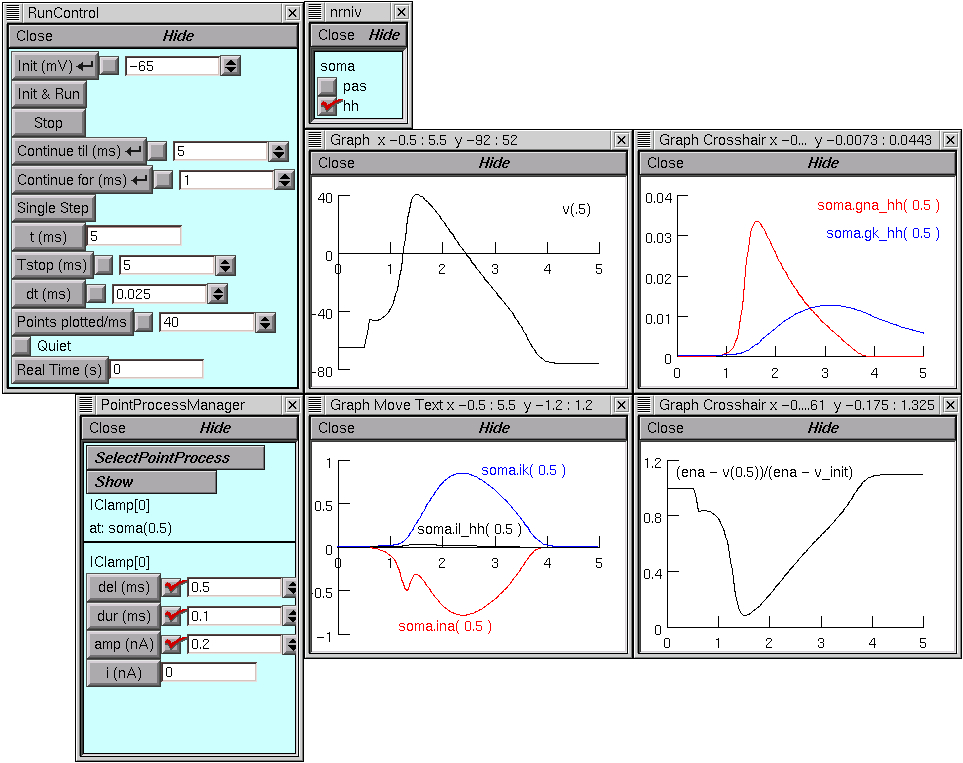
\includegraphics[height=\textheight,width=5in,keepaspectratio]{figures/neuron_gui.jpg}
\caption[The NEURON GUI \cite{brette2007simulation}]{The NEURON GUI showing the results of a simulation that has been run using the simulator\cite{brette2007simulation}.\label{fig:neuron_gui}}
\end{center}
\end{figure}

\begin{figure}
\begin{center}
\begin{lstlisting}
create soma, dend, dendx, axon
connect dend(0), soma(1)
connect dendx(0), soma(1)
connect axon(0), soma(0)

access soma
pt3dclear()
pt3dadd(0, 0, 0, 8)
pt3dadd(6, 0, 0, 18)
pt3dadd(10, 0, 0, 20)
pt3dadd(14, 0, 0, 18)
pt3dadd(20, 0, 0, 10)

insert hh
Ra = ra

dend {
  nseg = 21	// may need more
  diam = DEND_DIAM
  L = DEND_LENGTH

  insert hh
  gnabar_hh /= 5
  dend_gnabar_0 = gnabar_hh
  gkbar_hh /= 5
  Ra = ra
}
\end{lstlisting}
\caption[NEURON Hoc Example \cite{carenvale2006neuron}]{A code snippet from a Hoc script creating a neuron\cite{carenvale2006neuron}.\label{fig:hoc_example}}
\end{center}
\end{figure}

Another simulator, called GENESIS (GEneral NEural SImulation System)\cite{brette2007simulation}, is similar to NEURON in that it mostly models smaller neural networks including interactions within a single neuron\cite{bower1995book}. GENESIS uses a proprietary scripting language as well as formatted data files to create and run simulations. GENESIS can use MPI or PVM to parallelize its computations across multiple machines. Like NEURON, it can run simulations via a command-line interface known as G-Shell, a Python wrapper library, or a graphical user interface named XODUS\cite{brette2007simulation}. An example of the XODUS user interface can be found in Figure \ref{fig:genesis_gui} and a sample of the GENESIS scripting language can be found in Figure \ref{fig:gscript_example}\cite{bower1995book, brette2007simulation}.

\begin{figure}
\begin{center}
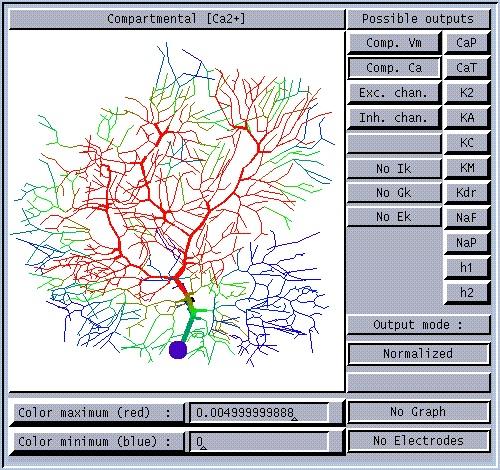
\includegraphics[height=\textheight,width=5in,keepaspectratio]{figures/genesis_gui.jpg}
\caption[The GENESIS GUI \cite{brette2007simulation}]{The GENESIS GUI (called XODUS) showing a visual representation of a Purkinje neuron model\cite{brette2007simulation}.\label{fig:genesis_gui}}
\end{center}
\end{figure}

\begin{figure}
\begin{center}
\begin{lstlisting}
create cell /n  
create segment /n/soma  
 
model_parameter_add /n/soma Vm_init -0.068  
model_parameter_add /n/soma CM 0.0164  
model_parameter_add /n/soma RM 1.500  
model_parameter_add /n/soma RA 2.500  
model_parameter_add /n/soma ELEAK -0.080  
 
model_parameter_add /n/soma LENGTH 4.47e-5  
model_parameter_add /n/soma DIA 2e-5  
 
runtime_parameter_add /n/soma INJECT 2e-9  
output_add /n/soma Vm  
 
run /n 0.05  
 
quit
\end{lstlisting}
\caption[GENESIS Script Example \cite{bower1995book}]{A code sample from a GENESIS script creating a neuron, injecting current into it, and outputting the voltage\cite{bower1995book}.\label{fig:gscript_example}}
\end{center}
\end{figure}

Unlike the NEURON and GENESIS simulators, the NEST (NEural Simulation Tool)\cite{brette2007simulation} simulator tends to focus on larger neural networks rather than smaller ones. NEST uses a command-line interface as well as a Python wrapper to create models and run simulations.  Unlike its counterparts, NEST lacks an out-of-the-box user interface component. Results of the simulation must be viewed using 3rd party Python libraries like matplotlib\cite{brette2007simulation}. An example of the NEST scripting language can be found in Figure \ref{fig:nest_script_example}\cite{gewaltig2007nest}.

The last simulator (and perhaps most-similar to NCS) that will be discussed is BRIAN. BRIAN is a neural simulator developed naively in Python and does not use a command-line intermediary: models are written exclusively in Python \cite{goodman2013brian}. BRIAN uses the scipy and numpy libraries to speed computations by taking advantage of native C code execution. It does not, however, provide the ability to parallelize the simulation across multiple machines. An example of a simple BRIAN simulation script can be found in Figure \ref{fig:brian_example}\cite{goodman2013brian}.

A comparison of these simulators and their features can be found in Table \ref{table:sim_comparison}\cite{hoang2013novel}.

\begin{figure}
\begin{center}
\begin{lstlisting}
/iaf_neuron Create /n1 Set
/iaf_neuron Create /n2 Set
/iaf_neuron Create /n3 Set
n1 n2 Connect
n1 n3 Connect
\end{lstlisting}
\caption[NEST Script Example \cite{gewaltig2007nest}]{A small code snippet of a NEST script creating three neurons and connecting them in a chain\cite{gewaltig2007nest}.\label{fig:nest_script_example}}
\end{center}
\end{figure}

\begin{figure}
\begin{center}
\begin{lstlisting}
from brian import *
eqs = '''
dv/dt = (ge+gi-(v+49*mV))/(20*ms) : volt
dge/dt = -ge/(5*ms) : volt
dgi/dt = -gi/(10*ms) : volt
'''
P = NeuronGroup(4000, eqs, threshold=-50*mV, reset=-60*mV)
P.v = -60*mV
Pe = P.subgroup(3200)
Pi = P.subgroup(800)
Ce = Connection(Pe, P, 'ge', weight=1.62*mV, sparseness=0.02)
Ci = Connection(Pi, P, 'gi', weight=-9*mV, sparseness=0.02)
M = SpikeMonitor(P)
run(1*second)
raster_plot(M)
show()
\end{lstlisting}
\caption[BRIAN Example \cite{goodman2013brian}]{An example of a BRIAN script creating a group of 4000 neurons and creating a raster plot from the result of the simulation\cite{goodman2013brian}.\label{fig:brian_example}}
\end{center}
\end{figure}

\begin{table}
\def\arraystretch{1.5}
{\tiny
\begin{tabular}{ l | p{0.5in} | p{0.5in} | p{0.60in} | l | p{0.70in} | p{0.5in} | p{0.50in} | p{0.4in} }
Simulator & Platform & Language & Coding Style & GUI & Realtime \newline Visualization & Neuron Models & Parallel Support & Python Interface \\
\hline
BRIAN & Linux Mac Windows & Python & Python & No & No & LIF HH IZH & None & Yes \\
\hline
GENESIS & Linux Mac Windows & C & C & Yes & No & HH & MPI PVM & No \\
\hline
NEURON & Linux Mac Windows & C C++ FORTRAN & HOC Python & Yes & No & HH LIF & MPI & Yes \\
\hline
NCS & Linux & C++ CUDA Python & Python & Yes & Under Development & HH LIF IZH & MPI GPU (ZeroMQ planned) & Yes \\
\hline
NEST & Linux Mac Windows & C++ Python & Python SLI & No & No & HH LIF IZH AdEx MAT2 & MPI & Yes \\
\hline

\end{tabular}
}
\caption[Simulator Comparison \cite{hoang2013novel}]{This table provides a comparison between the major neural simulators including NCS based on the features they provide users (modified from \cite{hoang2013novel}).\label{table:sim_comparison}\vspace{0.25in}}
\end{table}

\section{NCS}

NCS is a spiking neuron simulator that is written in C++ and CUDA. The simulator, similar to the BRIAN simulator discussed earlier, its currently focused on simulating large-scale neural networks, on the order of hundreds of thousands to millions of neurons and billions of synapses\cite{hoang2013novel, thibeault2011novel}. To handle these large-scale simulations, NCS is designed to scale to handle the sizable computational throughput needed. It is designed from the ground up to distribute the workload across multiple processors on multiple machines. In addition to using multiple CPU cores on each node, NCS also will detect and use NVIDIA GPUs if they are present on the machine to take advantage of the SIMD capabilities of these cards as well as their floating-point performance\cite{thibeault2011novel}.

Running on top of the C++ code is a thin Python layer that provides lower-level access to the simulator. This layer doesn't attempt to provide advanced capabilities in an effort to keep the C++ code as streamlined and as simple as possible without having to add additional overhead for higher-level functionality. For example, NCS doesn't explicitly provide any form of grouping or organization for the neurons it simulates. Rather, it keeps track of groups of neurons, individual neurons, and the connections between them. This may work for smaller simulations, but at the scale of millions of neurons and billions or trillions of synapses, this approach to organization would leave most users lost in their own design. Similarly, a thin python layer without programming conveniences like classes removes a level of abstraction that would be expected from a normal programmatic API. In addition, neuroscientists might like to avoid coding altogether and focus on the biology.

To provide an intuitive and modern way for neuroscientists to interact with the NCS simulator, a more capable and user-friendly interface needs to be created. Additionally, to make the simulator more extensible as a cluster-based neural simulator running large-scale models, a better method is needed to organize, create, run, manage, store, and report on simulations than running the simulation via a shell on the cluster and directly manipulating the filesystem. These characteristics of NCS and other neural simulators do not help them create collaborative environments where experiments can be shared, recreated, and verified. A better approach is needed to handling the many tasks that surround these simulators.

\section{Client-Server Model}

To solve these shortcomings, we have created a client-server based approach to the design of NCS. In this model of computing, a server running on a machine accepts requests from clients who wish to use the servers resources. A diagram of the client-server model can be found in Figure \ref{fig:client_server}\cite{wiki:clientserver}. In the context of NCS, the server will run on the master node of an NCS cluster and directly interface with the low-level Python interface. The server is responsible for multiple functions. Firstly, the server should be able to manage and keep track of the simulator. This includes calling NCS to run a simulation, ensuring that clients don't attempt to run a simulation while another is in progress, and managing the output of the simulator including resulting data, errors, warnings, and other messages as well as allowing clients to get access to this information. Using this computation model as opposed to the methods used by existing simulators provides a number of advantages. Firstly, the simulator can be used by multiple remote clients. This allows many different researchers to use the same cluster, and allows simulations to be run from non-console clients, such as a web browser. Secondly, it removes the need for direct shell access to the machine, which removes potential security risks associated with providing a remote shell. Lastly, it provides a centralized management system in which simulations can be logged, stored and shared in a consistent format, rather than the typical approach of allowing each user to create their own organizational methods. This makes it easier to share results, duplicate experiments, and incorporate models from other researchers into your own experiments.

\begin{figure}
\begin{center}
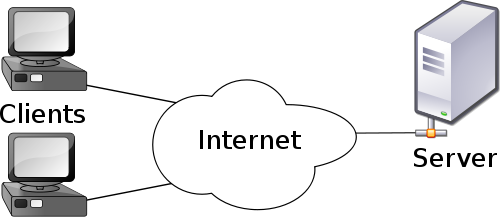
\includegraphics[height=\textheight,width=5in,keepaspectratio]{figures/client_server.png}
\caption[Client-Server Model \cite{wiki:clientserver}]{The client server model allows for multiple clients to request resources from the server\cite{wiki:clientserver}.\label{fig:client_server}}
\end{center}
\end{figure}

\section{HTTP \& REST}

\subsection{HTTP}

As a result of the client-server architecture chosen for NCS, a method is needed to transport information from the client to the server and vice versa. The HTTP protocol is a time-tested protocol used to transport textual and binary data over the Internet and various other computer networks. This makes HTTP an ideal candidate for handling the transfer of information between the client and server.

A HTTP transaction begins with a request from the client to the server. Each request can be one of four types: GET, POST, PUT, and DELETE. Each of these methods requests the server to perform a specific action on a target. The target of the action is specified as the \emph{path}. The path is specified like a UNIX filesystem path, in the form of a series of strings separated by forward slashes. The effect of actions GET, POST, PUT, and DELETE on a path are defined by the HTTP server itself, but generally follow a certain format\cite{fielding1999hypertext}. The GET method instructs the server that the client is requesting information about the path included in the request. For example, when visiting a website, a GET request to the path of / would ask the server to provide information pertaining to the index of the site, whereas a GET request to the path /blog would request information about the websites blog (provided such a path exists on the server). A POST request to /blog might instruct the server to create a new blog post with the data provided with the request (such as a title, author, and content).

Typically, when browsers interact with websites the data returned from the server is HTML, which the browser uses to render the page in the browser window. However, HTML is far from the only type of information that an HTTP response can contain. HTTP responses can contain plain text, binary data (including images), XML documents, JSON objects, or any other user-defined format. Following the standardization of HTTP/1.1 in 1999, which added the PUT and DELETE methods, HTTP became capable of performing all CRUD (Create, Read, Update, Delete) operations for persistent storage\cite{fielding1999hypertext}. The CRUD options of HTTP/1.1 form the basis of the REST architectural style\cite{fielding2000representational}.

\subsection{REST}

REST (REpresentational State Transfer) is an architectural pattern that defines a method of interaction between a client and server. The key component behind the REST architecture is the concept of a {\em{resource}}. A REST resource, in the context of HTTP, is a URI, or Uniform Resource Identifier. A URI for a web application is typically the location of the resource on the web server in the form of a URL or Uniform Resource Location\cite{fielding2000representational}. For example, the URI for the users resource might be http://example.com/users and a URI for a student who's student ID is 1033 might be http://example.com/student/1033. These URI's uniquely identify their respective resources on the servers they are hosted on as well as the Internet as a whole.

While the URI specifies a way to uniquely identify a resource, a method is needed to represent the resource\cite{fielding2000representational}. This is typically done using one of the formats mentioned in the previous section such as HTML, XML, or JSON. For example, a student resource might be represented in JSON format shown in Figure \ref{fig:json_example} or in an XML format such as in Figure \ref{fig:xml_example}. These formats provide a consistent method of interaction between client and server.

To interact with a RESTful interface in the context of HTTP, the client sends a request to a particular URI on the server with one of the HTTP methods mentioned previously. Sending a GET request tells the server that the client wishes to receive the representation of the resource it requested. If the client wished to receive the representation of the aforementioned student with ID 1033, it would send a GET request to the URI http://example.com/student/1033 and the server would respond with the information shown in Figure \ref{fig:json_example}. To add a student, the client would send a POST request to the server containing the representation of the student (in the same format as Figure \ref{fig:json_example}) directed at the URI corresponding to the new student's ID, say 1555, at http://example.com/student/1555. To update the student with ID 1555, the client would send a PUT request to the URI http://example.com/student/1555 with the updated user representation. Similarly, to remove the student, the client would send send a DELETE request to the URI http://example.com/student/1555. This architectural style makes a HTTP API standardized and predictable, making it easy for clients to interact with the server.

\section{The JSON Format}

There are several ways to transmit information over HTTP, some of which are discussed in the HTTP section of this chapter. The JSON (JavaScript Object Notation) format, as its name suggests, is derived from the Javascript syntax for an object. JSON, which was defined in 2001 by Douglas Crockford, is a textual format that takes a minimal approach to representing data\cite{bray2013json}. Unlike XML, JSON doesn't use opening and closing tags, but uses a list of properties instead, making the files smaller\cite{nurseitov2009comparison}. Additionally, JSON has several datatypes, which is a feature not present in XML, making it easily parsed into programming languages such as Python, Ruby, and Javascript, which usually require a single function call to turn a string of JSON into a language-native object. JSON also has a binary format called BSON that can be used to transfer and store information in a binary format that is more space conscious and holds a superset of the normal JSON data types\cite{chodorow2013mongodb}.

There are six data types available in the JSON format: number, string, boolean, array, object, and null\cite{bray2013json}. All strings in JSON are enclosed within double-quotes and are UTF-8 encoded. A JSON object is an associative array of name/value pairs, enclosed within curly braces. The names must be strings followed by a colon and then the value. The key/value pairs are delimited by commas. Numbers are decimal numbers that can be in E notation or fractional. Arrays are lists of values within square brackets delimited by commas. Boolean values are simply true and false, and null is represented as the text null. An example JSON document using all types is shown in Figure \ref{fig:json_all_types}.

\begin{figure}
\begin{center}
\begin{lstlisting}
{
    "name": "Bob",
    "grade": "sophomore",
    "age": 24,
    "phone": "1+(775)555-5555"
}
\end{lstlisting}
\caption[JSON User Example]{This figure shows how a user might be defined using the JSON format. The student contains four attributes. Name, grade, and phone are string attributes, whereas age is a numerical attribute.\label{fig:json_example}}
\end{center}
\end{figure}

\begin{figure}
\begin{center}
\begin{lstlisting}[language=XML]
<student>
    <name>Bob</name>
    <grade>sophomore</grade>
    <age>24</name>
    <phone>1+(775)555-5555</phone>
</student>
\end{lstlisting}
\caption[XML Example]{This figure shows how a user might be defined using the XML format. Like the JSON example in Figure \ref{fig:json_example}, this student object contains four elements. XML doesn't provide the ability to dictate the type of elements, so all elements contain strings.\label{fig:xml_example}}
\end{center}
\end{figure}

\begin{figure}
\begin{center}
\begin{lstlisting}
{
    "company_name": "Planetary Express",
    "phone": "1+(800)555-5555",
    "manager": "Hubert Farnsworth",
    "company_net_worth": 0.0,
    "personnel": [
        "Phillip J. Fry",
        "Turanga Leela",
        "Hermes Conrad",
        "Amy Wong",
        "John Zoidberg",
        "Scruffy",
        "Bender Rodriguez"
    ],
    "total_deliveries": 100,
    "website": null,
    "is_profitable": false
}
\end{lstlisting}
\caption[JSON All Types]{This figure shows all valid JSON types. company\_name is a string, personnel is an array, total\_deliveries is a numerical value, website is a null value, and is\_profitable is a boolean value.\label{fig:json_all_types}}
\end{center}
\end{figure}

\section{WebSockets}

HTTP is a request-response protocol. It does not provide a method of streaming data between the client and server in a full-duplex fashion like that of TCP. To solve this problem, a new protocol was created that allows full-duplex communication via HTTP called WebSockets. WebSockets allow Javascript running on the client's browser to initiate a connection with a server in which both the client and the server can send data to one another simultaneously\cite{fette2011websocket}. This is helpful in many different applications where it would not be desirable to continuously request data from the server (polling) when there may not be any data that the client needs. When using WebSockets, the client can simply wait until the server has data to send and receive it asynchronously without constantly polling the server for it. This greatly reduces the network footprint of real-time HTTP-based applications and provides a much more intuitive interface for the exchange of data between client and server when such situation arise. For example, a web-based instant messaging client could use WebSockets to wait for incoming messages from the server and receive them as soon as they are ready, as opposed to constantly polling the server many times per second to check for new messages.

\section{MongoDB}

In recent years, a number of new database systems have been developed that do not rely on the traditional relational-model, which often use SQL as their database language. These databases are colloquially known as NoSQL databases in reference to the fact that they do not use SQL as a data management language\cite{lith2010investigating}. MongoDB is one of these databases. Instead us using tables and columns like in a traditional database it uses collections and documents\cite{chodorow2013mongodb}. Documents are JSON objects that are stored in a BSON format on disk. A collection is a list of documents, usually with a similar format (but this is not required). This type of database is advantageous because it doesn't require a strict schema with each attribute in its own column like in a SQL database\cite{chodorow2013mongodb}. This allows more flexibility in the way you want to store and retrieve your data. For example, storing the data shown in Figure \ref{fig:json_all_types} would require a few different tables in a well-designed SQL database. MongoDB becomes even more advantageous when the data your application works with is already in a JSON format. MongoDB uses Javascript as the language to manage the database data, which provides methods for CRUD operations as well as a few aggregate functions such as summation and average. More complicated queries require the use of a MapReduce programming model\cite{chodorow2013mongodb}. Database ORMs exist in many languages for MongoDB, so often times the user will never need to use Javascript to interact with the database and can use the language of their choice. Python contains a a library called MongoKit that performs this task\cite{tsoukalos2014using}.

\section{Client-Side Web Development}

\subsection{Bootstrap}

Over the years, the Internet and the World Wide Web have seen a massive expansion in size, ubiquity and utility. As the World Wide Web evolves, the way websites are built and designed also continues to evolve. Originally, websites were designed by hand and often took an exorbitant amount of time to design and implement. Adding to the problem, different browsers render web pages differently; even when the code is exactly the same, the differences can often times be dramatic. To combat this, a number or tools and frameworks have come about that aim to be both easy to use and cross-browser compatible\cite{lerner2012forge}. One of these frameworks is Bootstrap. 

Originally developed by Twitter for creating a consistent UI for internal tools, Bootstrap is a front-end framework that provides design templates that work across browsers and for various screen sizes (including mobile) and aims to provide a clean and aesthetic user interface. Web page elements such as forms, buttons, headers, tables, navigation, alerts, panels and numerous others are included in the Bootstrap package so developers don't have to create and style them themselves. Bootstrap includes a number of Cascading Style Sheet (CSS) rules to create and style the widgets and elements on the page, as well as a small amount of Javascript to make some of the elements interactive, such as the accordion component that shows and hides different panels in an accordion-like fashion. An example of a web page created with Bootstrap is shown in Figure \ref{fig:bootstrap_web_page} and some of the components Bootstrap contains can be found in Figure \ref{fig:bootstrap_components}\cite{bootstrap2014}.

\begin{figure}
\begin{center}
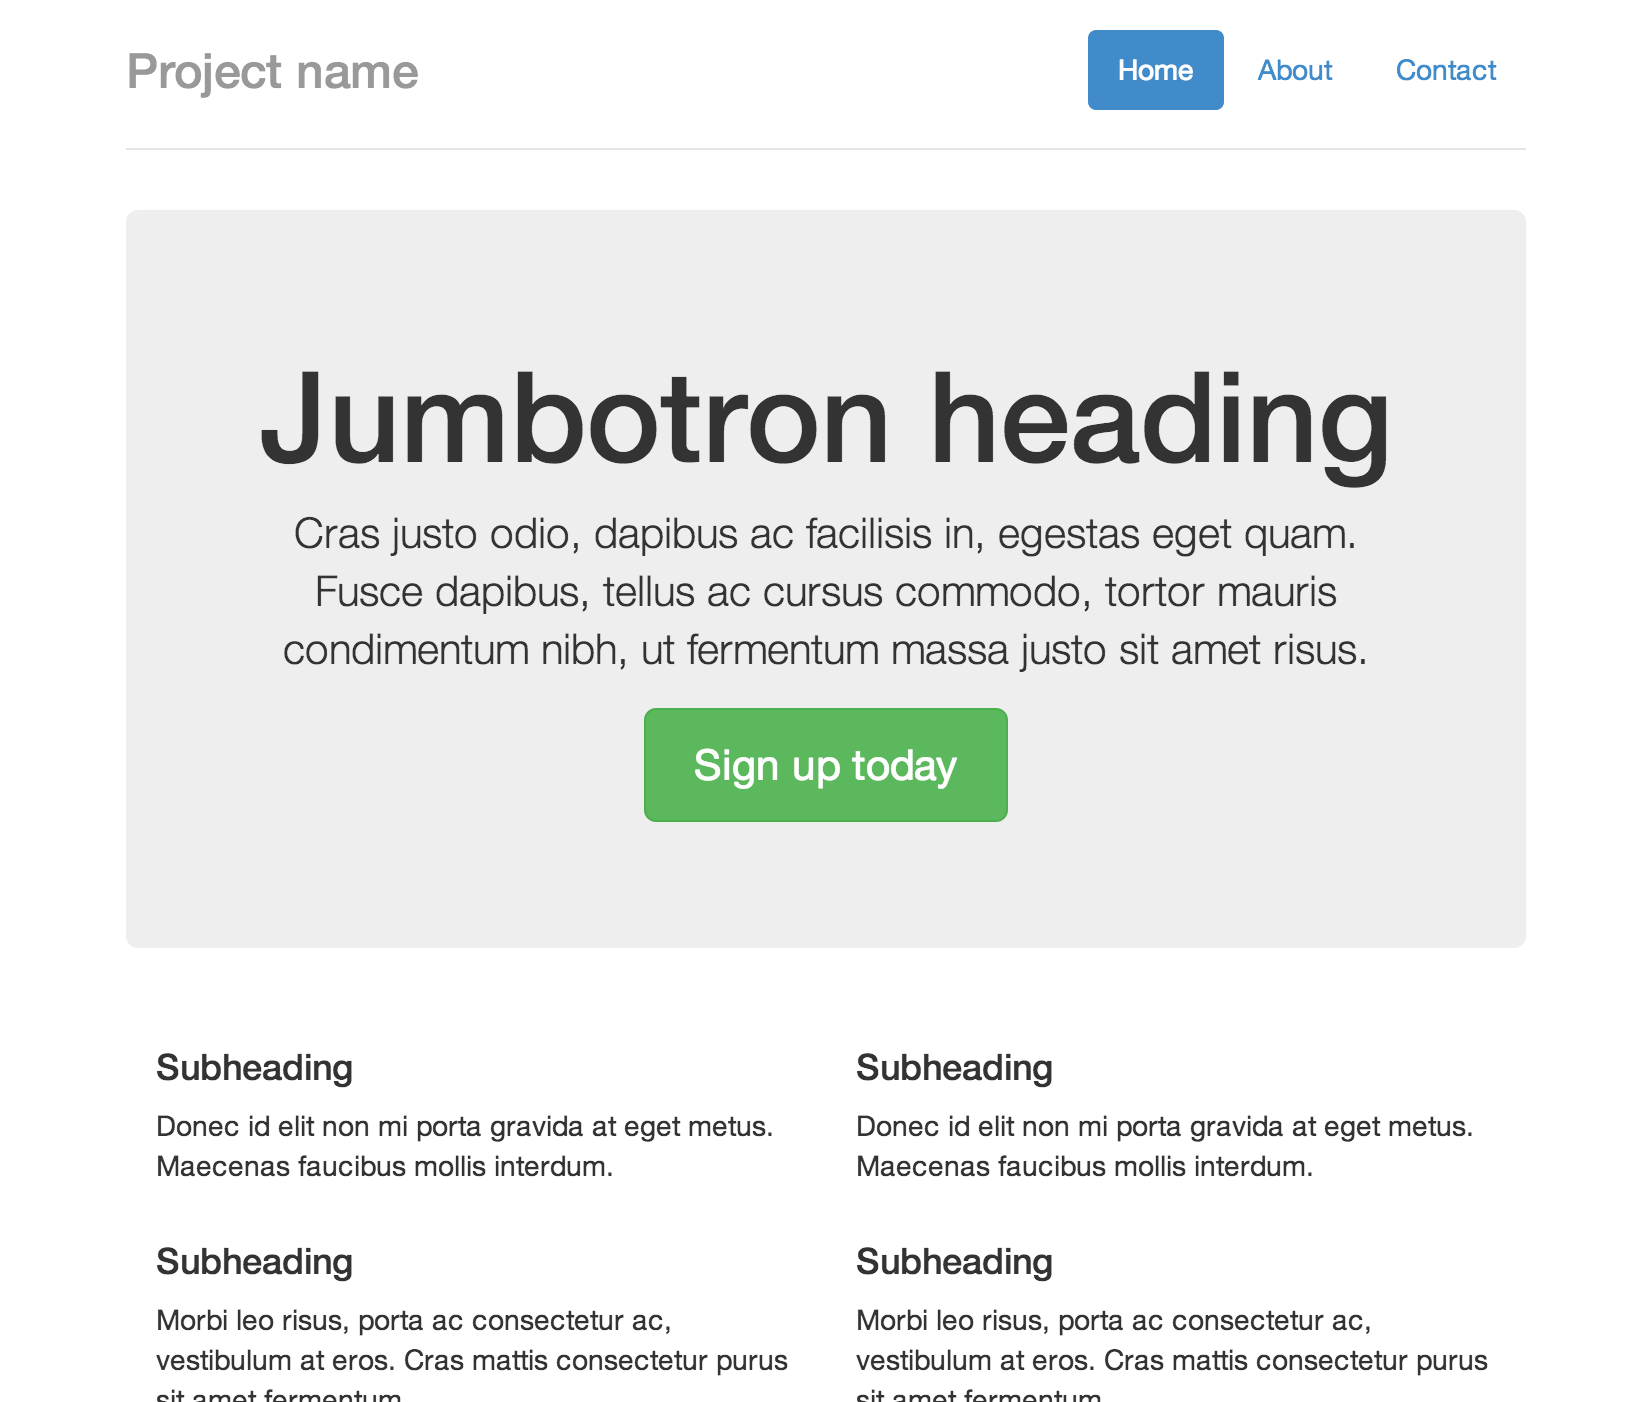
\includegraphics[height=\textheight,width=5in,keepaspectratio]{figures/bootstrap.png}
\caption[Bootstrap Web Page \cite{bootstrap2014}]{This is a simple example page that was created with the Bootstrap front-end framework. The page contains a navigation bar, page header, jumbotron component, and several paragraph elements that stack if the browser window becomes small enough\cite{bootstrap2014}.\label{fig:bootstrap_web_page}}
\end{center}
\end{figure}

\begin{figure}
\begin{center}
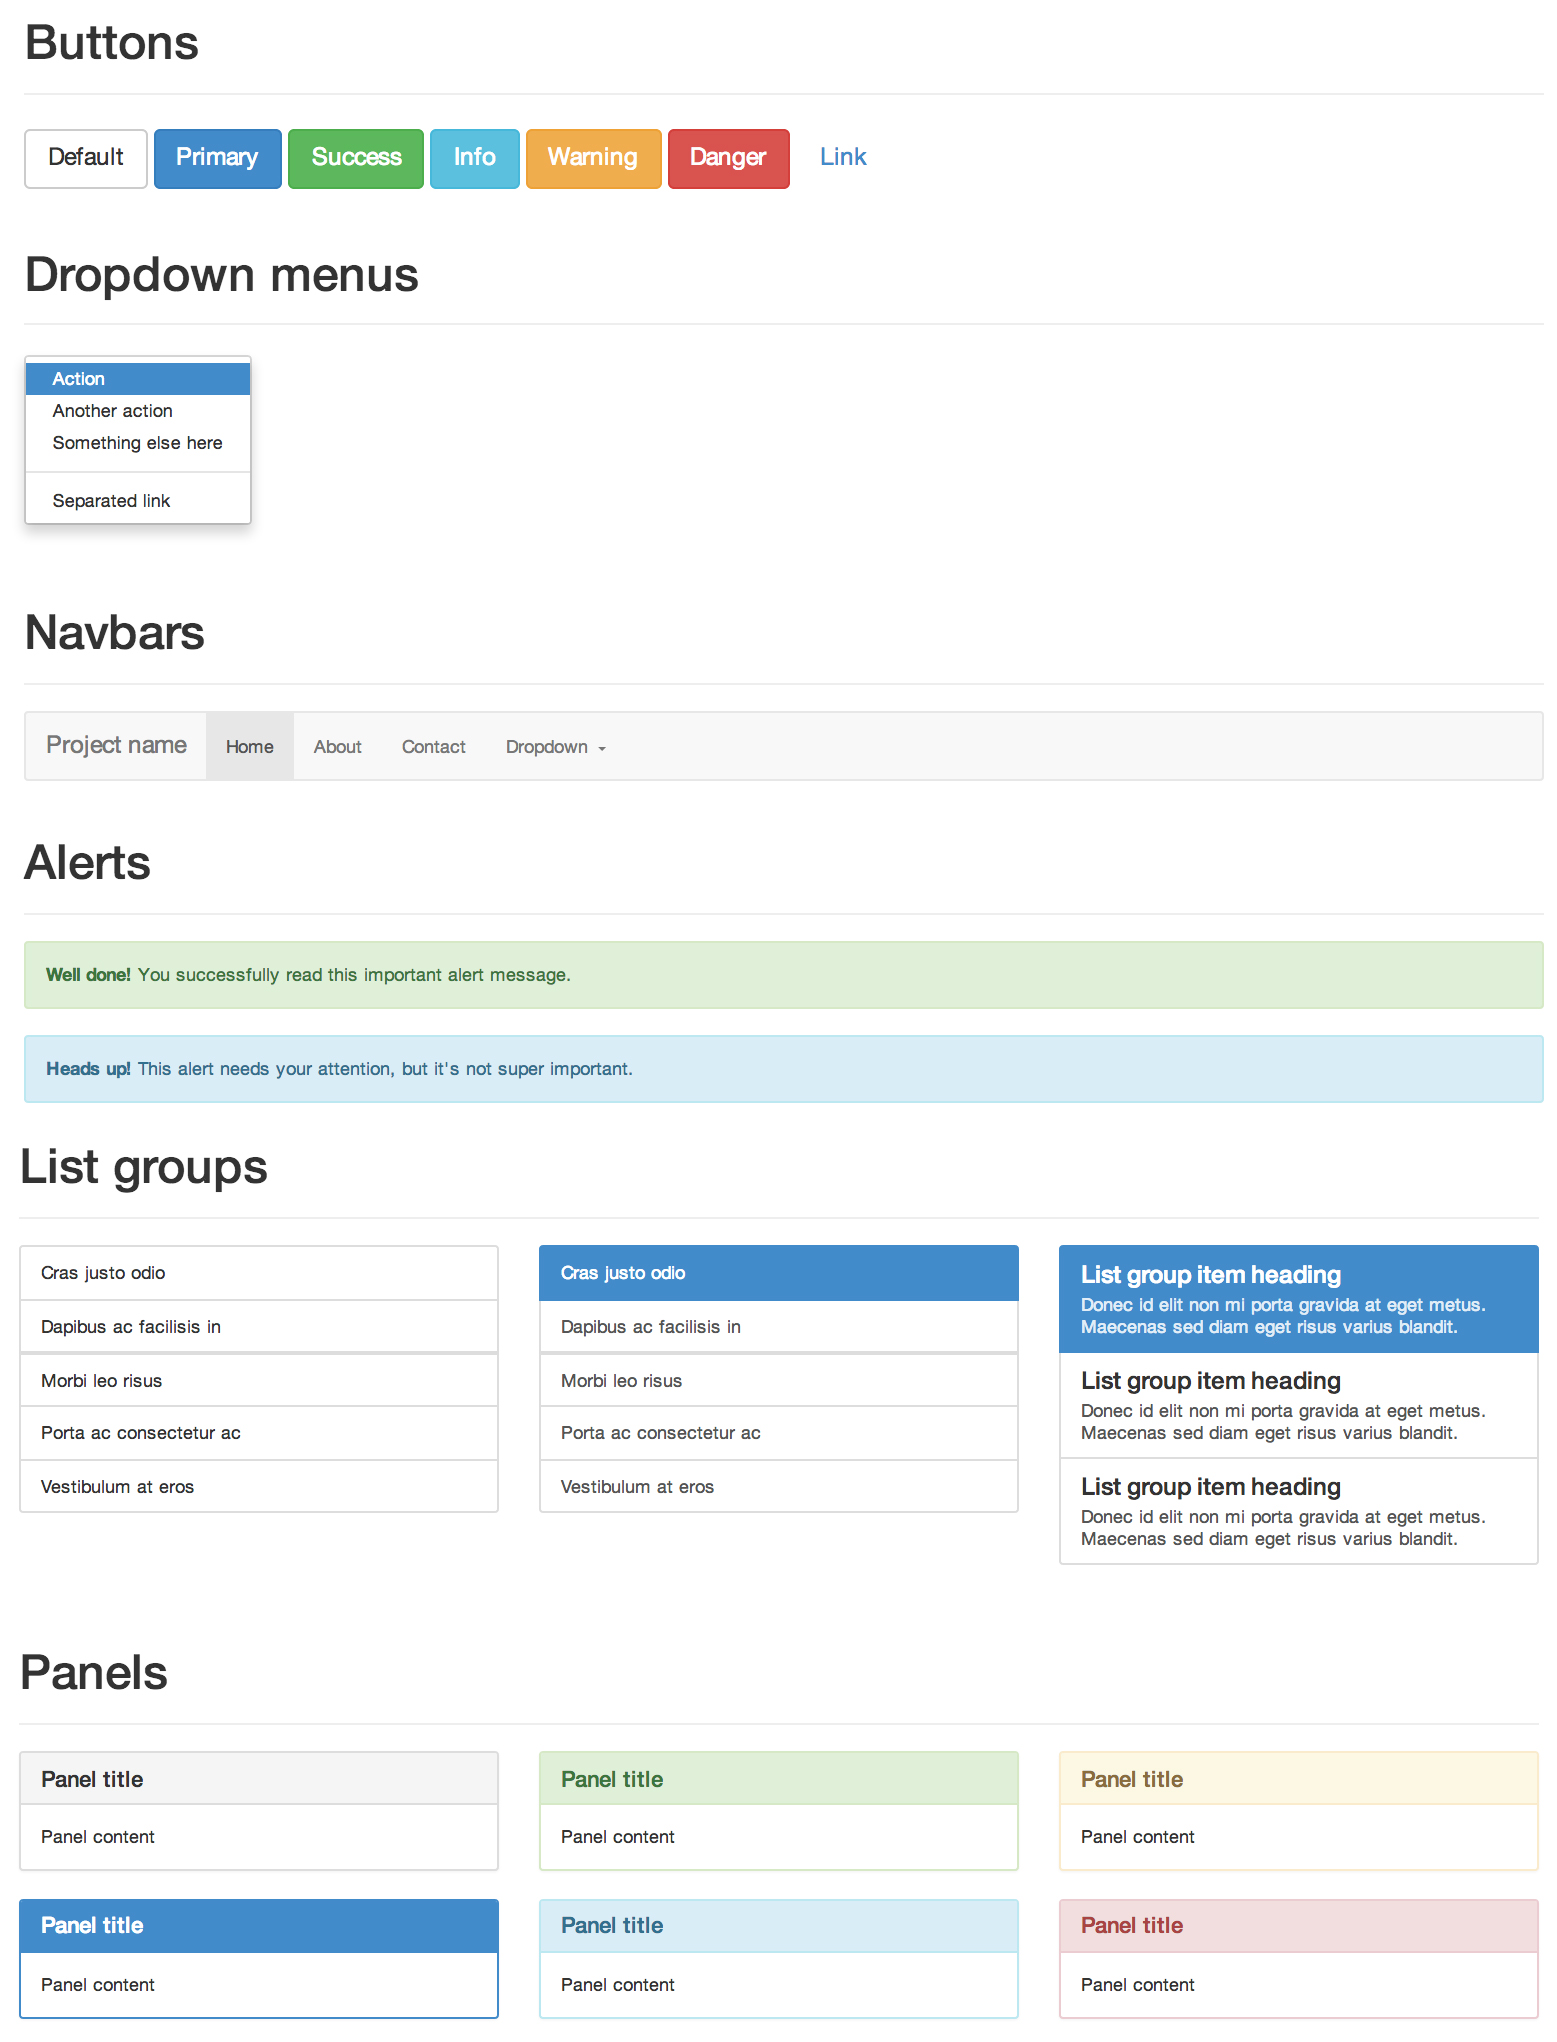
\includegraphics[height=\textheight,width=5in,keepaspectratio]{figures/bootstrap_components.jpg}
\caption[Bootstrap Components \cite{bootstrap2014}]{This figure shows several more Bootstrap components that are available for use in web applications\cite{bootstrap2014}.\label{fig:bootstrap_components}}
\end{center}
\end{figure}

\subsection{AngularJS}

While Bootstrap changes the way we create the look and feel of websites, AngularJS changes how we make web pages dynamic. Traditionally most of the code front-end developers would write involves directly manipulating the elements on the HTML page when data changes or the user interacts with the application. Most of this kind of development is tedious, and writing the code for it takes time away from other tasks that are central to the functionality of the application. Angular removes the need to write the code that manipulates the elements on the web page and allows developers to focus on the background tasks that need to be performed such as fetching data from a server\cite{darwin2013angularjs}. It does this by providing developers a way to create declarative-style directives in the HTML of the web page. An example of this would be rendering elements from a list on the page, such as a list of books. As books are added, deleted, and modified from a list in an Angular Javascript module, they are automatically updated on the web page instantly. This is a possible due to Angular's two-way data binding concept that is at the core of its functionality. As a result of the two-way data binding feature, any changes to the view are reflected in the model of the application, and any changes in the model are reflected in the view. A diagram illustrating this two-way data binding can be found in Figure \ref{fig:angular_data_binding}\cite{angularconcepts2014}. If you compare this with a traditional web application using jQuery to manipulate the DOM, you can see that the complexity of accomplishing a two-way data binding would greatly increase and would require you to write a lot more code. An example comparing the code required for each of these approaches can be found in Figure \ref{fig:jquery_example} and Figure \ref{fig:angular_example}.

Angular also provides a \emph{resource} module that allows developers to easily interact with RESTful interfaces. For each resource only requires a location be specified in the form of a URL where the resource can be found. Other options may be provided to enhance the behavior of the resource object in the event custom functionality may be needed, or in other cases when a list of objects might be returned instead of just a single object. This makes it trivial to create a Javascript application that interacts with a RESTful web application. An example of creating and using an Angular resource can be found in Figure \ref{fig:angular_resource}.

\begin{figure}
\begin{center}
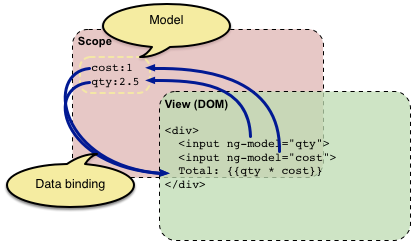
\includegraphics[height=\textheight,width=5in,keepaspectratio]{figures/angular_data_binding.png}
\caption[Angular data binding \cite{angularconcepts2014}]{This figure illustrates the concept of Angular's data-binding feature. Changes to the scope's cost and qty variables are automatically propagated to the view without any further action required by the developer. If the user changes the values in the input areas on the web page, those changes are automatically reflected in the scope variables as well\cite{angularconcepts2014}.\label{fig:angular_data_binding}}
\end{center}
\end{figure}

\begin{figure}
\begin{center}
\begin{lstlisting}
$.ajax({
  url: '/message_list',
  success: function (data, status) {
    var result = JSON.parse(data);
    for (var i = 0; i < result.length; i++) {
      $('ul#log').append('<li>' + result[i].msg + '</li>');
    }
  }
});
\end{lstlisting}
\begin{lstlisting}[language=HTML]
<ul class="messages" id="log">
</ul>
\end{lstlisting}
\caption[JQuery DOM Manipulation]{This Javascript snippet uses JQuery to perform an HTTP request to get some data from the server and add it to an HTML list. The Javascript code is highly dependent on the HTML code. The {\em{}`ul\#log'} provides a specific HTML element to add the element to. What if the data needed to be used in another HTML element? We would need to modify the request function.\label{fig:jquery_example}}
\end{center}
\end{figure}

%%%%%%%%%%%%%%%%%%%%%%%%%%%%%%%%%%%%%%%%%%%%%%%

\begin{figure}
\begin{center}
\begin{lstlisting}
$http( '/message_list' ).then( function ( response ) {
  for (var i = 0; i < response.length; i++) {
    $scope.log.push( response[i] );
  }
});
\end{lstlisting}
\begin{lstlisting}[language=HTML]
<ul class="messages">
    <li ng-repeat="entry in log">{{ entry.msg }}</li>
</ul>
\end{lstlisting}
\caption[Angular DOM Manipulation]{This Javascript snippet uses Angular to perform an HTTP request to get some data from the server and add it to an HTML list. The data being retrieved has no ties to the HTML code at all. In the HTML, we add an angular directive (ng-repeat) to loop over the list of messages and add the elements dynamically.\label{fig:angular_example}}
\end{center}
\end{figure}

\begin{figure}
\begin{center}
\begin{lstlisting}
var User = $resource('/user/:userId', {userId:'@id'});
User.get({userId: 1155}, function(user) {
  $scope.users.push(user);
});
\end{lstlisting}
\begin{lstlisting}

\end{lstlisting}
\caption[Angular Resource Module]{This figure demonstrates Angular's resource module. This module allows Angular to easily interact with RESTful web servers. The developer defines the Angular resource using the URL of the resource on the server. Once the resource has been defined, the developer can query the RESTful interface using the resource object.\label{fig:angular_resource}}
\end{center}
\end{figure}


  \chapter{Design \& Implementation}
\label{chapter:design}

\section{NCS Software}

The NCS simulator provides the ability to simulate biologically-realistic neural interactions at a large scale. While NCS performs the core goals of a brain simulator, there is a much larger set of functionality that is needed for a simulator than running the simulation itself. This functionality includes building the simulation, running the simulation, storing simulation data, and analyzing results, which is imperative to the researcher using any brain simulator. We designed a suite of tools that surround the NCS simulator that provide users the ability to perform these tasks. These tools include a consistent storage and management system for the simulations users create, a programmatic Python interface, a web-based interface for building, running and analyzing simulations, and a way to visualize the results of the simulation. With the construction of these tools we have also introduced a new architectural concept, the client-server model, that is unique to current brain simulators. A diagram showing a high-level overview of NCS and its surrounding software can be found in Figure \ref{fig:ncs_architecture}

\begin{figure}
\begin{center}
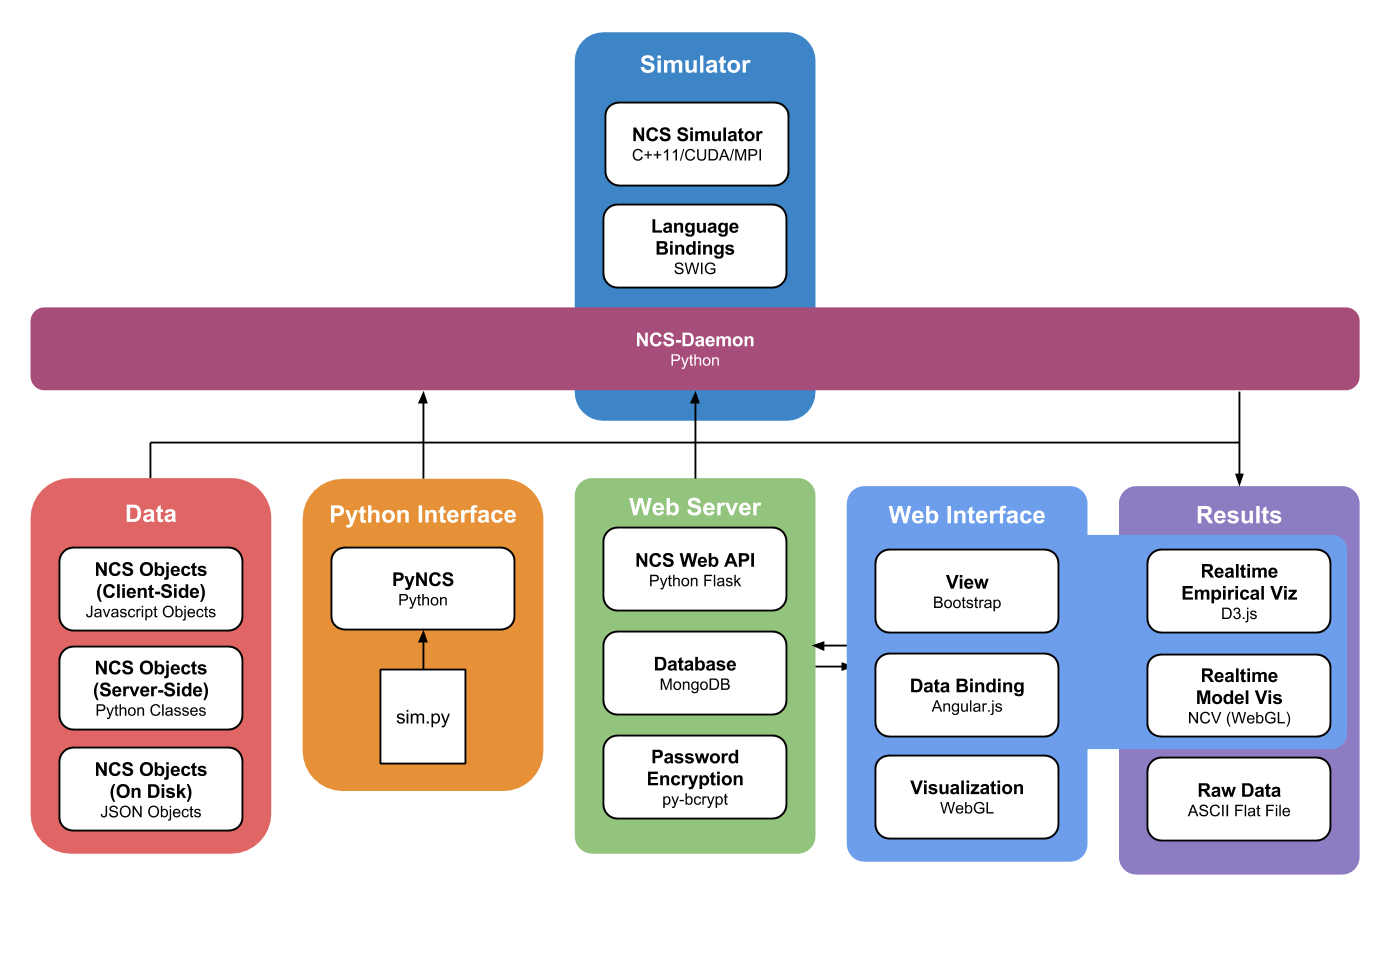
\includegraphics[height=\textheight,width=6in,keepaspectratio]{figures/ncs_architecture.png}
\caption[NCS Architecture]{This diagram is a graphical representation of the NCS software suite. The simulator performs the core simulation tasks and is shown in dark blue. NCS-Daemon acts as a intermediary between external services and the simulator and provides a single point of entry for all simulator tasks. It allows NCS to focus on being as fast as possible by handling the organizational outside the simulator codebase. The tools that surround the simulator include a Python interface, and a web interface. These services interact with NCS-Daemon to gain access to the simulator.\label{fig:ncs_architecture}}
\end{center}
\end{figure}

\section{NCS-Daemon}

Part of the goal in designing NCS was to provide the simulator as a service that multiple clients could interact with rather than as a program that is run from the command line. To do this, a process or daemon must be consistently running on the root node of the NCS cluster that accepts connections from clients attempting to use the simulator. Additionally, a method of transport is needed to carry information to the daemon from the clients and vice versa. As discussed earlier, one of the best methods to transfer textual data over a network is the HTTP protocol. HTTP is ubiquitous and libraries exist for using it in virtually every programming language, making it an easy choice for implementing the communication fabric between the daemon and the clients. Finally, HTTP is a client-server-based protocol, which suits the goal of the project perfectly.

There are a myriad of different libraries and frameworks to choose from to create a server using HTTP as the underlying protocol. Since the low-level simulator functions are exposed using a thin Python layer, it makes sense to choose a Python-based HTTP library to handle the connections to the simulator. Several popular libraries exist as Python modules: the most popular of which is Django\cite{googletrends2014django}. Django is a so-called full-stack web application framework, as it has facilities for creating database entities, an administrative interface, form-validation, and many other features that make it advantageous to use as a general web application framework. NCS-Daemon, however, would not make use of the vast majority of these features, making Django superfluous for the requirements of the application. Another web framework called Flask\cite{grinberg2014flask} provides a more minimal set of functionality. It provides the ability to designate \emph{routes} that call certain Python functions when a request comes in to a certain URI, making it very easy to implement a REST interface. Flask also has a host of extensions that help extend the functionality of the application including WebSockets and integration with MongoDB, a popular JSON-based NoSQL database. Because of its simplicity and extensibility, we chose to implement the daemon using the Flask web application framework. A simple "Hello, world" Flask application can be found in Figure \ref{fig:flask_hello_world}.

\begin{figure}
\begin{center}
\begin{lstlisting}[language=Python]
from flask import Flask
app = Flask(__name__)

@app.route("/")
def hello():
    return "Hello World!"

if __name__ == "__main__":
    app.run("localhost", 8000)
\end{lstlisting}
\caption[Flask Hello World]{This Flask application serves the plain text "Hello World" when an HTTP client sends a GET request to the '/' route.\label{fig:flask_hello_world}}
\end{center}
\end{figure}

To design NCS-Daemon as a RESTful service, a number of resources needed to be defined. The first resource is the \emph{simulator} resource. The \emph{simulator} resource refers to the current status of the simulator. A GET request to this resource will provide information on the status of the simulator, a POST request containing simulation data will attempt to start a new simulation, and a DELETE request will attempt to stop the currently running simulation. The next resource is the \emph{simulation} resource. The simulation resource refers to a specific simulation created by a user. This resource allows the GET and DELETE methods. The GET method returns information about the simulation specified, including log information, reports related to the sim, and the simulation object that was run by the simulator. A DELETE request to a specified simulation resource will delete that simulation, as well as any data associated with it. The next resource is the \emph{report} resource. The \emph{report} resource requests the contents of a report generated by a previous simulation. It accepts the GET and DELETE methods, which instruct the server to provide the report, and remove the report from disk respectively. In the event a report was specified as a streaming report meant for WebSockets, the resource will return an error. The final resource is the \emph{login} resource. This resource provides an endpoint for users to authenticate with the server which is an important component of NCS-Daemon.

When implementing any network-based application, security is always a matter of concern, especially when the application is facing the Internet. Preventing unauthorized use of the NCS simulator and protecting user information are the main problems with regard to application security. To prevent unauthorized use of the simulator a login system was created. To use the simulator, the user must have an account on the server. Next, before any interaction with the daemon, the user must first send a POST request to the \emph{/login} route on the server, supplying their username and password. In response, the server sends an authorization token specific to that user. Each request to the server must contain this authorization token in the HTTP headers or the server will reject the request as unauthorized. By providing the token to users, it prevents their credentials from being passed with each request. If an attacker were to begin intercepting communications between the client and server after the user has logged in, he would only gain the access token. The attacker would still be able to gain access to the simulator for a certain time, but the user's credentials would remain secret and could not be used to gain access to external accounts such as email and bank accounts registered using the same password. To completely protect access to the simulator and the users credentials, the connection to the server must be made over HTTPS using SSL or TLS, which are used to create a completely secure connection that cannot be decoded by other parties during or after transmission.

NCS-Daemon is implemented as a RESTful interface and as such exposes these resources to clients in the form of routes. In addition to the traditional RESTful routes exposed by the application, NCS-Daemon also has two different WebSocket routes that are also available for streaming live data to the client provided the client has a library to interact with the WebSocket protocol. The routes exposed by NCS-Daemon as well as their descriptions and allowed methods can be found in Table \ref{table:routes}.

\begin{table}
\def\arraystretch{1.5}
\begin{tabular}{ l | p{0.75in} | p{3.2in} }
Route & Methods & Resource Description \\
\hline
/login & POST & The login route accepts requests containing a username and password and responds with an access token provided the credentials were correct.  \\
\hline
/simulator & GET POST DELETE & The simulator route provides a resource for the state of the simulator. A GET request returns information about the current status of the simulator. A POST request will instruct the daemon to start a simulation. Finally, a DELETE request instructs the daemon to cancel the current simulation.  \\
\hline
/simulation/:id & GET DELETE & The simulation route provides a resource for past simulations. A GET request returns information about the simulation requested. A DELETE request instructs the daemon delete the specified simulation.  \\
\hline
/report/:id & GET & The report route provides the report generated by a simulation, including whether it can be streamed through a WebSocket.  \\
\hline
/report\_stream/:id & WebSocket & The report\_stream route is used for streaming live report data over a WebSocket interface.  \\
\hline
/geometry\_stream & WebSocket & The geometry\_stream WebSocket can be used to stream the locations and geometry of neurons and connections for a realtime visualization.  \\
\end{tabular}
\caption[REST Interface Routes and Descriptions]{This table shows the routes, methods and descriptions for NCS-Daemon's RESTful interface.\label{table:routes}\vspace{0.25in}}
\end{table}

NCS-Daemon is designed to be fully testable and is designed with good software engineering practices. The project repository is hosted on GitHub and is integrated with the Travis Continuous Integration service. This service runs the project's tests each time a developer attempts to update the repository and alerts the user when their changes break the tests. Additionally, the service outputs the code coverage of the tests, which measure the amount of code in the repository was run during the tests, which keep track of how effective the testing suite is. Ideally, this number should be as close to 100\% as possible. The software class diagram for NCS-Daemon can be found in Figure \ref{fig:ncs_daemon_diagram} and the GitHub repository showing the NCS-Daemon README with the testing and coverage badges can be found in Figure \ref{fig:readme}.

\begin{figure}
\begin{center}
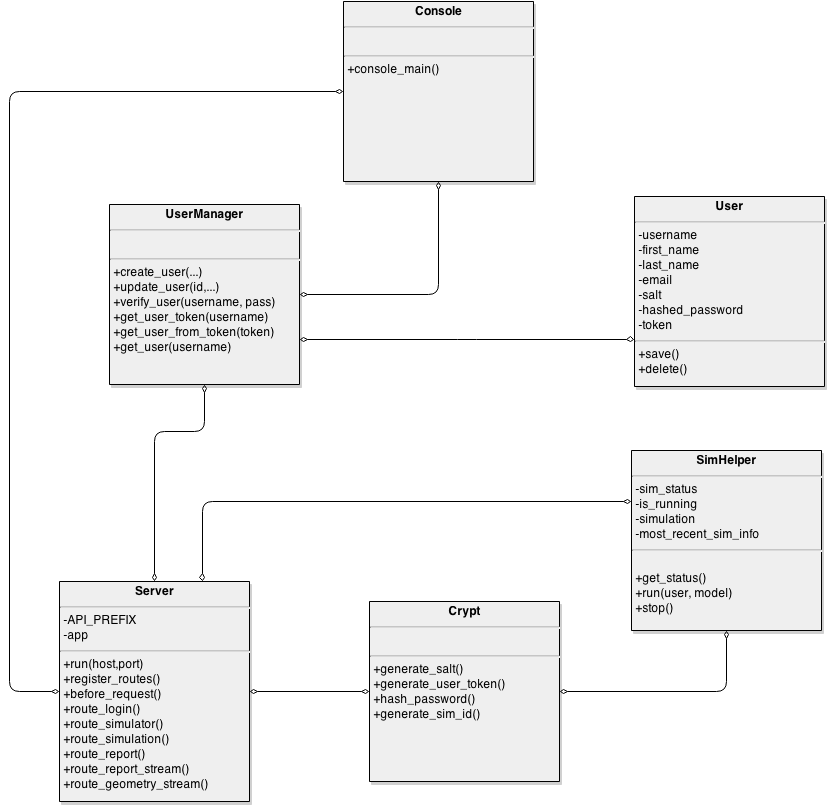
\includegraphics[height=\textheight,width=6in,keepaspectratio]{figures/ncs_daemon_diagram.png}
\caption[NCS-Daemon Class Diagram]{This is the NCS-Daemon's class diagram with testing components omitted.\label{fig:ncs_daemon_diagram}}
\end{center}
\end{figure}

\begin{figure}
\begin{center}
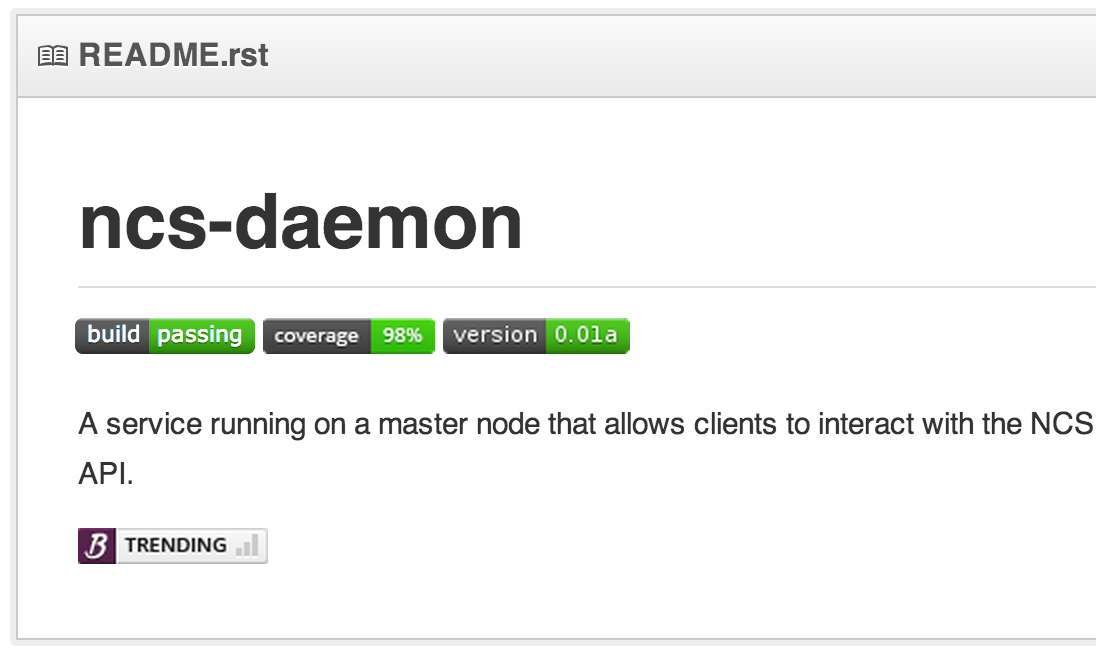
\includegraphics[height=\textheight,width=5in,keepaspectratio]{figures/readme.png}
\caption[NCS-Daemon GitHub README]{The README file for NCS-Daemon contains badges that link to the current testing state of the project, including if its tests are passing, and what the code coverage percentage is.\label{fig:readme}}
\end{center}
\end{figure}

\section{Simulation Concepts \& Transfer Format}

NCS simulations are defined as a hierarchical structure of groups and neuron groups as well as several other entities each with their own parameters. These entities include neurons, synapses, stimuli, reports, neuron\_aliases, and synapse\_aliases. Neuron entities contain the model used to calculate whether or not a neuron will fire on a particular time tick. Neurons can be of several types, each with their own set of parameters that affect the behavior of the neuron. Currently, the simulator supports Leaky-Integrate-and-Fire (LIF), Hodgkin-Huxley, and Izhikevich models for neurons. Synapses define the properties of connections between neurons including synaptic learning and plasticity. Stimuli define where electrical current will be applied during the simulation and how it should be delivered. Reports define which properties and which neurons or synapses should be collected and either streamed over a WebSocket or written to disk during the simulation. Lastly, neuron\_aliases and synapse\_aliases provide a way to refer to large collections of neurons or synapses under a single name instead of all their collective names, reducing the work required for referencing large groups or neurons or synapses.

Since NCS doesn't have native support for higher-level constructs, a system needed to be developed allows for users to organize the groups of cells more effectively. To accomplish this, we created a hierarchical system of groups as a way to structure the model. A group may contain multiple types of entities, the first of which are subgroups. Subgroups are instances of other groups placed within a larger group that have a label that distinguishes themselves from other subgroups in the same group. Groups can also contain neuron groups, which are simply collections of neurons of the same type that act as a single unit. Groups are also where connections are defined. A connection is created between two neuron groups with a synapse type and a certain probability of connection between them. Finally, aliases are created within groups. Aliases allow a single label to refer to multiple objects. For example, if there are two neuron groups labeled "A" and "B", then a neuron alias named "AB" could be created that refers to both of these subgroups. This system allows users to better organize their models, and create larger models more effectively than creating numerous unorganized neuron groups. This system of organization is illustrated in Figure \ref{fig:group_diagram}.

\begin{figure}
\begin{center}
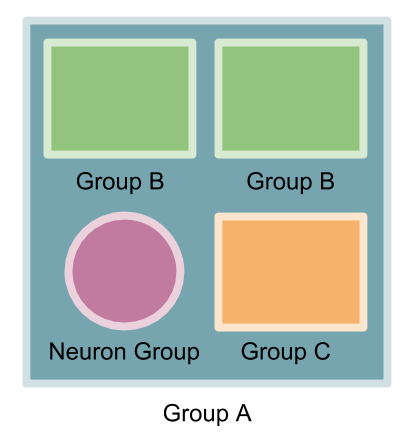
\includegraphics[height=\textheight,width=5in,keepaspectratio]{figures/group_diagram.png}
\caption[Group Hierarchy Diagram]{This diagram shows a visual representation of a group in NCS. Group A contains two instances of Group B, a neuron group, and another group, Group C. A JSON representation of a group can be found in Figure \ref{fig:group_json}.\label{fig:group_diagram}}
\end{center}
\end{figure}

In order to transfer and store simulations, some kind of textual representation for the simulation model and its entities must be created. Due to the hierarchical nature of the simulation model, with simulations possibly containing many of the same group type, the tree of groups could grow at a sizable rate if this structure were fully expanded into JSON. This makes the size of the files much larger, which is bad for both transporting the JSON over a network or storing it on disk. Additionally, it makes decoding the simulation once it reaches the daemon more complicated and slow due to the redundant information and very deep model structure. To combat this, we have implemented a normalized approach to storing the data in a textual format, akin to the concepts of a relational database. Instead of expanding the simulation tree into its full form, the tree is traversed and groups are added to a list of groups. Inside the groups, rather than expanding subgroups into their corresponding JSON, we maintain a reference to the other group in the form of a unique identifier, that is generated randomly. This saves space by reducing redundancy that would be common in many models. Since the other entities are not defined in a hierarchical fashion, they do not need to be normalized and can be added to a list with other entities of the same type. A template showing the simulation transfer format with normalized groups can be found in Figure \ref{fig:empty_transfer_format}.

\begin{figure}
\begin{center}
\begin{lstlisting}
{
    "top_group": "5728ec1d381bad25744bc54c42ba425",
    "neurons": [
    
    ],
    "synapses": [
    
    ],
    "stimuli": [
    
    ],
    "reports": [
    
    ],
    "groups": [
    
    ],
    "neuron_aliases": [
    
    ],
    "synapse_aliases": [
    
    ]
}
\end{lstlisting}
\caption[JSON Transfer Format]{The JSON transfer format without any entities defined. The \emph{top\_group} property specifies the id of the topmost group in the simulation heirarchy. When a client submits a simulation to NCS-Daemon the arrays would be populated with data.\label{fig:empty_transfer_format}}
\end{center}
\end{figure}

In addition to their specifications, entities also contain metadata that describes information about the entity, such as its type, name, description, author, institution, and author's email. When stored on disk or in a database such as MongoDB, this metadata can be used to determine where a model was created, who it was created by, and which scientific papers it might have been created for or from. This will aid researchers in collaborating on experiments, and keeping models organized. An example of an Izhikevich neuron entity including its metadata can be found in Figure \ref{fig:izh_json} and a group entity with subgroups, neuron groups, aliases, connections and metadata can be found in Figure \ref{fig:group_json}.

\begin{figure}
\begin{center}
\begin{lstlisting}
{
    "_id": "c4f5ea85f4c5ae86c4ebc4a854",
    "entity_type": "neuron",
    "entity_name": "neuron_izh_1",
    "description": "This is an extended description of the entity",
    "author": "Nathan Jordan",
    "author_email": "njordan@cse.unr.edu",
    "specification": {
        "type": "izhikevich",
        "a": 0.02,
        "b": 0.2,
        "c": -65.0,
        "d": 8.0,
        "u": -12.0,
        "v": -65.0,
        "threshold": 30
    }
}
\end{lstlisting}
\caption[JSON Izhikevich neuron model]{An Izhikevich neuron model with metadata represented in JSON. The metadata surrounds the Izhikevich parameters contained within the specification object.\label{fig:izh_json}}
\end{center}
\end{figure}

\lstset{
  basicstyle=\tiny\ttfamily
}

\begin{figure}
\begin{center}
\begin{lstlisting}
{
    "_id": "df90sahf0sd9ha8sdhf8dhsa",
    "entity_type": "group",
    "entity_name": "BasalGanglia",
    "description": "This is an extended description of the entity",
    "author": "Nathan Jordan",
    "author_email": "njordan@cse.unr.edu",
    "specification": {
        "geometry": {
            "width": 100.0,
            "height": 200.7,
            "depth": 300.3
        },
        "subgroups": [
            {
                "group": "sdfh8ahsdf80has0d89fh0as9dhf",
                "label": "striatum",
                "location": {"x": 123.5, "y": 456.5, "z": 789.5}
            },
            {
                "group": "hf8as0df8asdhf80ahsd80f",
                "label": "pallidum",
                "location": {"x": 2354.5, "y": 456.5, "z": 543.5 }
            }
        ],
        "neuron_groups": [
            {
                "neuron": "hfd80sahs80dhf0shda90fhshdf",
                "label": "gpe",
                "count": 400,
                "geometry": {"width": 100.4, "height": 200.7, "depth": 300.8},
                "location": {"x": 234.9, "y": 456.4, "z": 543.2}
            },
            {
                "neuron": "hasd890fhas80fhas80dhf",
                "count": 30,
                "label": "gpi",
                "geometry": {"width": 100.1, "height": 200.6, "depth": 300.7},
                "location": {"x": 784.4, "y": 926.1, "z": 999.2}
            }
        ],
        "neuron_aliases": [
            {
                "alias": "gpx",
                "labels": ["gpe", "gpi"],
                "aliases": ["an_alias"]
            }
        ],
        "synaptic_aliases": [
            {
                "alias": "sample_synapse_alias",
                "labels": ["GP_synapse"]
            }
        ],
        "connections": [
                {
                    "presynaptic": "gpe",
                    "postsynaptic": "gpi",
                    "probability": 0.5,
                    "synapse": "hfd8nfiodnsa80dbhfbas80df",
                    "recurrent": false
                }
        ]
    }
}
\end{lstlisting}
\caption[JSON Group Definition]{JSON Group specification with metadata parameters.\label{fig:group_json}}
\end{center}
\end{figure}

\lstset{
  basicstyle=\footnotesize\ttfamily
}


\section{PyNCS}

Now that the server and transfer schema have been defined, there needs to be a convenient way to interact with the server without having to deal with HTTP and the JSON representation during transfer. To address this, we have created a Python library called PyNCS. PyNCS allows users to communicate with an NCS server using an intuitive Python interface. To connect to the server, the user instantiates a \emph{Simulator} object with their username and password. If the library fails to connect to the simulator, an authentication exception is thrown. An example showing the usage of the simulator via PyNCS can be found in Figure \ref{fig:simulator_connection}. Models are created using Python classes that are defined in the PyNCS package. These classes provide a way to create models in an object-oriented fashion without use of dictionaries or less-structured Python types. When creating entity objects, the parameters are checked against a known list of acceptable parameters for that entity as to prevent mistakes when creating a model, and alerting the user to their mistakes before the simulation is run, so they can more easily identify where the error is and fix it quickly. For example, creating an Izhikevich neuron and specifying \emph{x} as a parameter will throw an exception. An example of this functionality can be found in Figure \ref{fig:pyncs_izh}.

\begin{figure}
\begin{center}
\begin{lstlisting}[language=Python]
# Correct
server = Simulator(
    host='ncscluster.example.edu',
    port=8081,
    username='my_username',
    password='my_password'
)

# Throws ConnectionError
server = Simulator(
    host='no_ncsdaemon_here.example.edu',
    port=8081,
    username='my_username',
    password='my_password'
)

# Throws AuthenticationError
server = Simulator(
    host='ncscluster.example.edu',
    port=8081,
    username='my_username',
    password='not_my_password'
)
\end{lstlisting}
\caption[PyNCS Simulator Example]{This example gives three different scenarios for connections. The first example results in a successful connection, the second example attempts to connect to a host where NCS-Daemon is not running, and the last example attempts to connect to NCS-Daemon with the incorrect credentials.\label{fig:simulator_connection}}
\end{center}
\end{figure}

\begin{figure}
\begin{center}
\begin{lstlisting}[language=Python]
# This successfully defines an Izhikevich neuron
izh = IzhNeuron(
    a=0.5,
    b=0.5,
    c=0.5,
    d=8.0,
    u=-12.0,
    v=Normal(-65.0, 0.5),
    threshold=30.0
)

# This throws an EntityError because we tried to specify x
izh = IzhNeuron(
    a=0.5,
    b=0.5,
    c=0.5,
    d=8.0,
    u=-12.0,
    x=10.0,
    threshold=30.0
)
\end{lstlisting}
\caption[PyNCS Izhikevich Model]{This figure shows how an Izhikevich neuron would be declared in PyNCS. The first example successfully creates an Izhikevich neuron type, whereas the second example results in an exception.\label{fig:pyncs_izh}}
\end{center}
\end{figure}

The Python classes also enforce which parameters are required and optional. This allows users to only specify which parameters that are pertinent to the entity they are creating without specifying extra parameters that are empty. This makes PyNCS code more readable by reducing a level of verbosity, makes the code faster to write, and keeps code size to a minimum.

Once the model and other entities have been created, the user must create a \emph{Simulation} object. The simulation object encapsulates a single instance of a simulation. The most important service the \emph{Simulation} object performs is maintaining references to the reports generated by the simulation. These reports can be downloaded to the client from the server for further processing, visualization or anything else the user might wish to use the simulation data for. They are not downloaded automatically due to the possibility that the reports can become quite large dependant on the number of neurons or synapses being reported on and the frequency at which data on these entities is collected. The \emph{Simulation} object can also be used as a WebSocket client to stream realtime data from the server. Lastly, the simulation object contains diagnostic information and log data related to the simulation so the user can view and address any potential problems that may arise during a simulation. The \emph{Simulation} object can only be used for one simulation; to create and run another simulation, an additional \emph{Simulation} object must be create. An example of a \emph{Simulation} object being created and run can be found in Figure \ref{fig:pyncs_run_sim}.

\lstset{
  basicstyle=\tiny\ttfamily
}

\begin{figure}
\begin{center}
\begin{lstlisting}[language=Python]
izh = IzhNeuron(
    a=0.5,
    b=0.5,
    c=0.5,
    d=8.0,
    u=-12.0,
    v=Normal(-65.0, 0.5),
    threshold=30.0
)
syn = FlatSynapse(
    delay=10.0,
    current=60.0
)
nrn_grp1 = NeuronGroup(
    neuron=izh,
    count=30,
    label="izh1",
    geometry=Geometry(),
    location=Location()
)
nrn_grp2 = NeuronGroup(
    neuron=izh,
    count=50,
    label="izh2",
    geometry=Geometry(),
    location=Location(),
)
conn = Connection(
    presynaptic="izh1",
    postsynaptic="izh2",
    probability=0.5,
    synapse=syn
)
grp = Group(
    entity_name="my_group",
    subgroups=[],
    neuron_groups=[nrn_grp1, nrn_grp2],
    neuron_aliases=[],
    synapse_aliases=[],
    connections=[conn]
)
stim = RectCurrentStimulus(
    amplitude=3.0,
    width=2,
    frequency=10,
    probability=0.6,
    time_start=0,
    time_end=1,
    destinations=["my_group:izh1"]
)
rpt = Report(
    report_method=Report.METHOD_FILE,
    report_type=Report.TYPE_NEURON,
    report_target=[nrn_grp1],
    probability=0.5,
    time_start=0.0,
    time_end=1.0
)
sim = Simulation(
    top_group=grp,
    stimuli=[stim],
    reports=[rpt]
)
server = Simulator(
    host='ncscluster.example.edu',
    port=8081,
    username='my_username',
    password='my_password'
)

if server.get_status() == Simulator.IDLE:
    server.run(sim)
\end{lstlisting}
\caption[PyNCS Running Simulation]{This figure shows how a simulation would be created and run in PyNCS. The sim object is created using the top-level model and a list of stimuli and reports. The Simulator object is created using a hostname and port as well as a username and password which establishes a connection to NCS-Daemon. Once a connection has been established, the status of the simulator can be checked. If the simulator is idle, we can run the created simulation.\label{fig:pyncs_run_sim}}
\end{center}
\end{figure}

\lstset{
  basicstyle=\footnotesize\ttfamily
}

\section{Web Interface}

While the PyNCS interface provides a way for users with knowledge of programming (specifically Python programming) to create and run simulations programmatically, this is a skill set that many potential neuroscientists using the NCS simulator may not have or want to exercise. To address the needs of all neuroscientists, a more user-friendly and less-technical interface is needed to interact with the brain simulator. Simulators such as NEURON and GENESIS discussed in the background section use old interfaces developed for native windowing environments like X11. The problem with these interfaces is that they are now antiquated, as newer technologies exist to create these environments for modern operating systems. Additionally, they must be run on the users computer directly, forcing them to install software on their machine which may not be desirable. To address these problems, we have created a web-based interface that acts as a client to the NCS-Daemon server and allows neuroscientists to create simulations using only a web browser.

To create the web interface we took advantage of a couple tools that would greatly reduce design time. Firstly, we used the Bootstrap front-end framework to create a consistent look and feel, and save a lot of development time by not having to develop custom UI widgets. Secondly, we made use of AngularJS as the Javascript framework powering the page. Angular allows easy integration with the DOM without having to directly manipulate it as well as providing a way to easily interact with the RESTful interface of NCS-Daemon. Currently, there are five tabs in the NCS Web Interface: model builder, sim builder, reports, model database, and robot simulator. 

The model builder, shown in Figure \ref{fig:model_builder}, is a graphical way for users to create their models. The design of the model builder posed some particularly difficult UI design challenges. While some entities like neurons are single-layer entities, group entities form a hierarchical structure that could be several layers deep. Users need to be able to navigate efficiently through these levels and do so without feeling like the UI has become too cluttered. We felt that a tree-type interface would lead to too much clutter and greatly degrade user experience. To develop a more effective interface, we took some queues from file explorers of different operating systems. File explorers also work on a hierarchical data set (a filesystem is a tree) and have been developed to make it easy for users to navigate around the filesystem and perform operations on it. A particular example of this is the Windows Explorer interface that uses breadcrumbs to show the user where they are and a main content area where the content of the location is displayed. 

\begin{figure}
\begin{center}
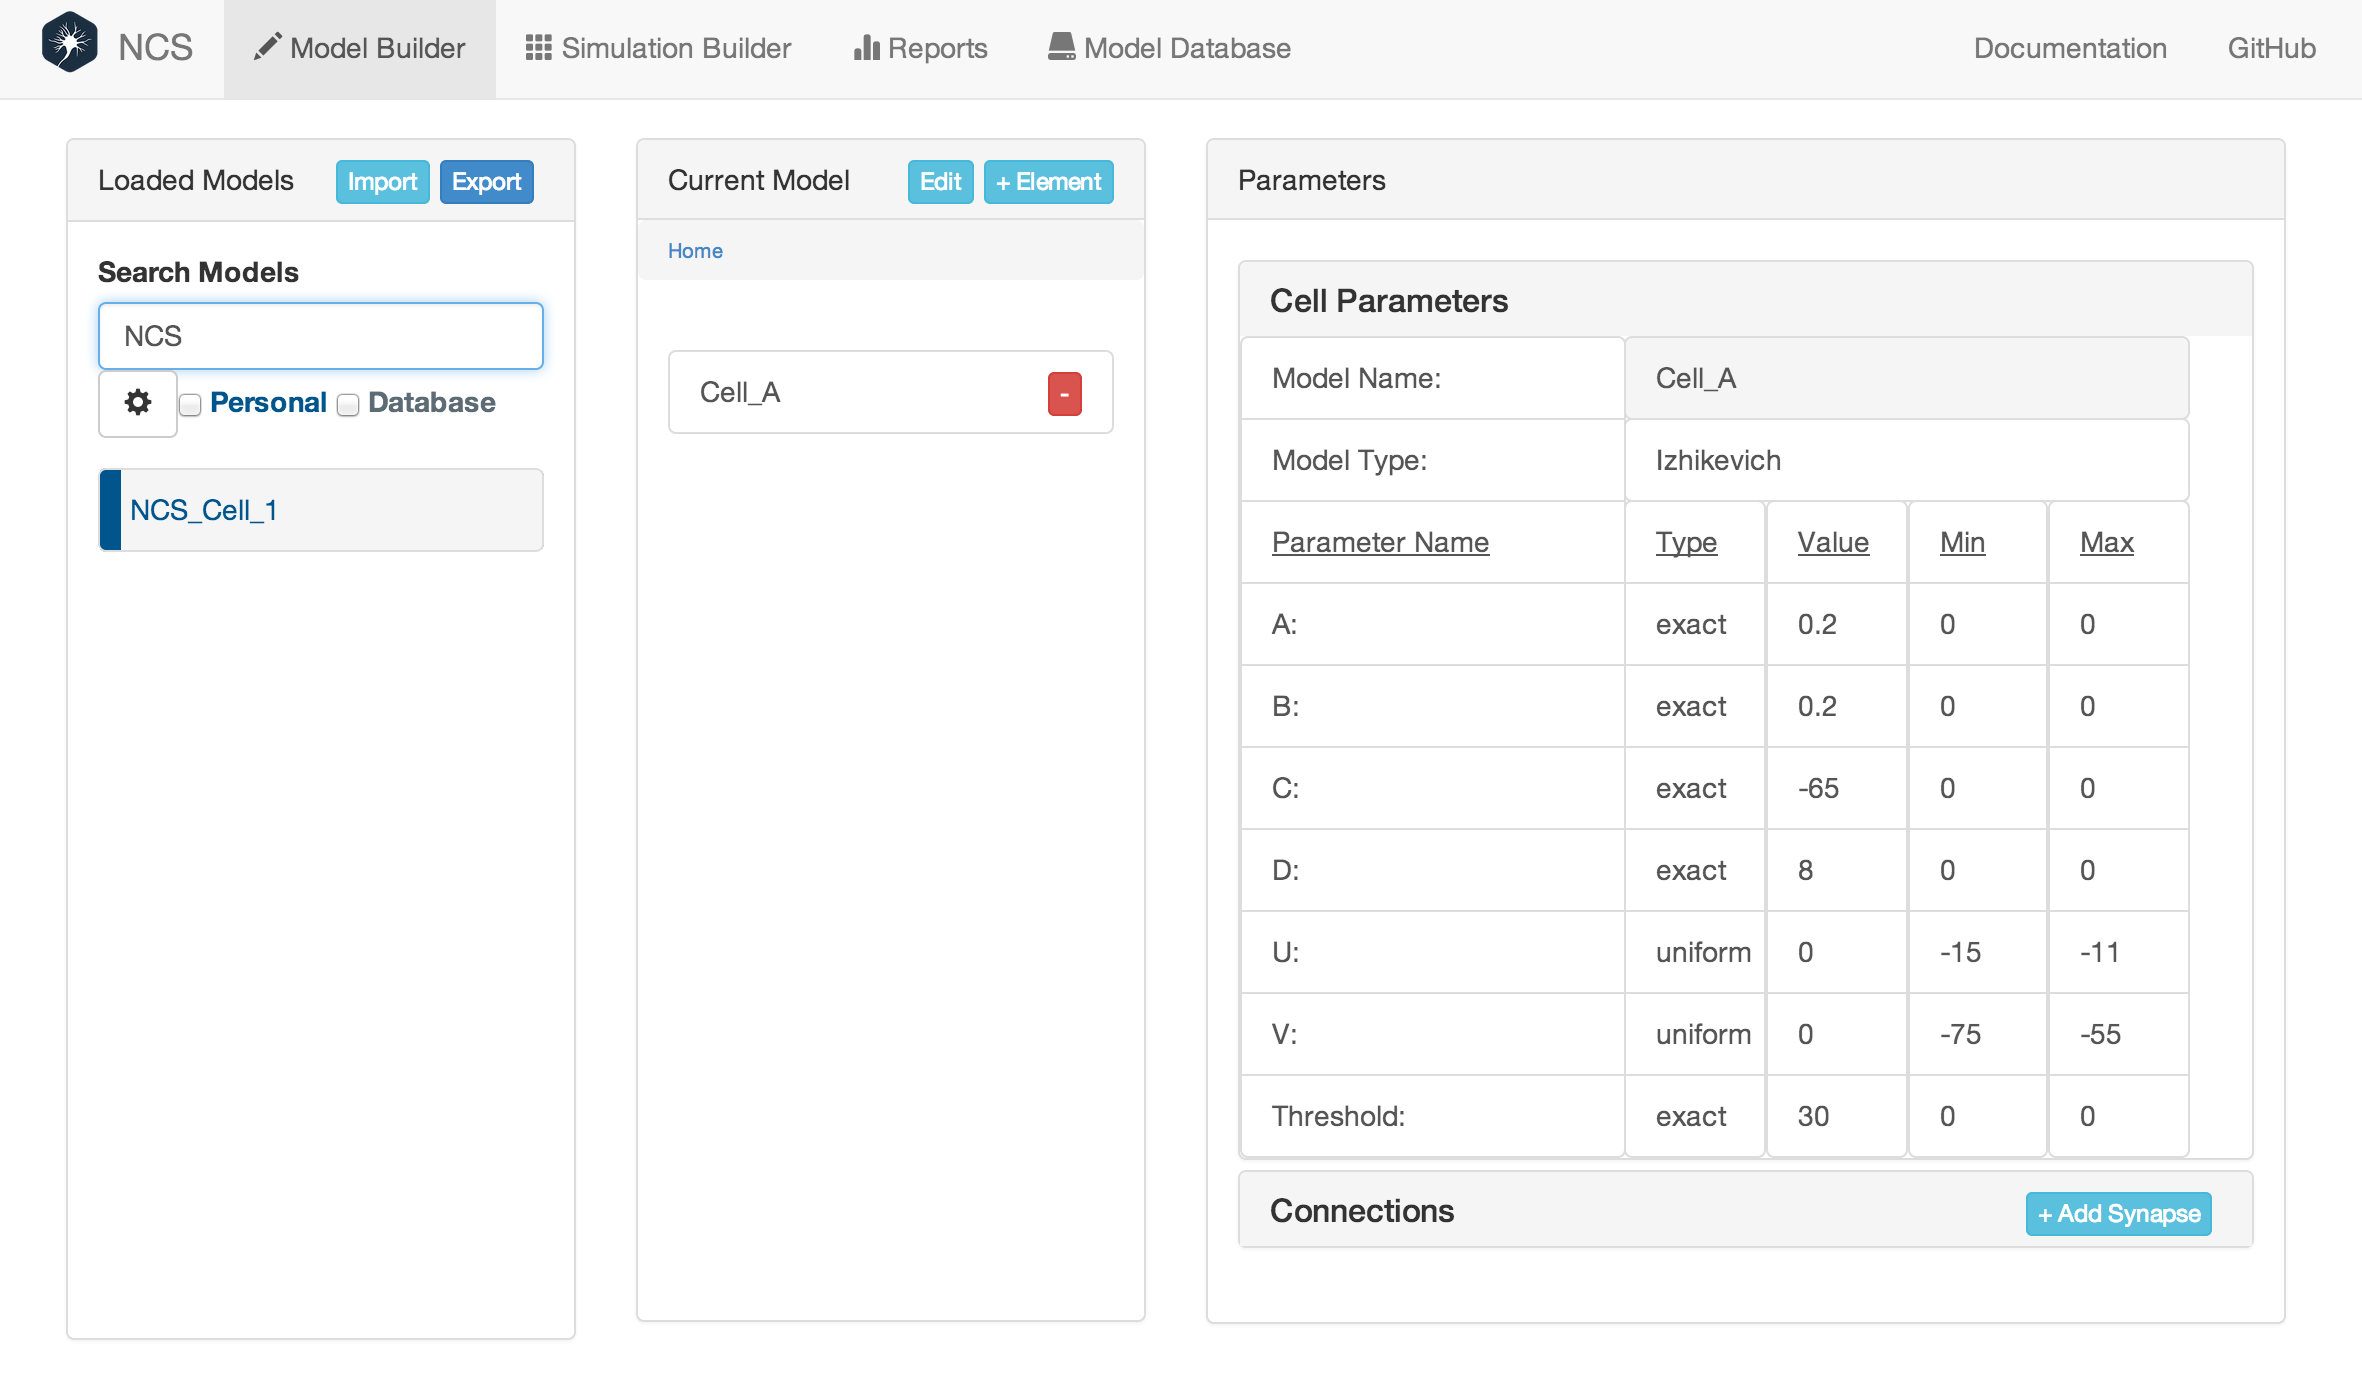
\includegraphics[height=\textheight,width=5in,keepaspectratio]{figures/model_builder.png}
\caption[Model Builder]{The model builder is organized into three sections split vertically across the page. The leftmost panel contains models that the user has built or loaded from a file or database. The second panel displays entities that are within the currently active group. The rightmost panel displays parameters of a selected entity. In this case, it is displaying the Izhikevich parameters for Neuron\_1.\label{fig:model_builder}}
\end{center}
\end{figure}

In our design, we implemented a system in which breadcrumbs are used to navigate the tree and keep track of where the user is in the hierarchy (similar to file explorer) and a content area in the form of a panel updates as the user navigates. As the user moves through the groups they are creating, links are created and removed along a top bar that indicates where they are in the model. If they want to move to a different position in the hierarchy, they simply click the link corresponding to the name of the group they want to move to and the content area updates accordingly. In the content area is a list of subgroups the user can further navigate into. When the user selects one of these subgroups a new subgroup is created, the user is shown the contents of the new subgroup (when created it is empty) and a breadcrumb is added to the list. 

The rightmost panel is where model specifications are created. This panel lets the user modify the properties of entities they have selected. For example, if the user were to select a neuron from the model selection list on the left parameters related to the neuron would be editable to the user on the right panel, such as the voltage threshold or resting potential. Values updated here are propagated to the back-end model and are updated there.

Once the user has created or imported the model they wish to execute in the simulator, they then switch to the sim builder tab. The sim builder tab, shown in Figure \ref{fig:sim_builder} allows the user to create interactions with the model that they have built and actually create the simulation. Firstly, the user should create at least one stimulus to inject into a select group of cells within the model to bring it to life. The stimulus can be generated from a few different sources, including a file-based stimulus, or a socket-based stimulus. The socket-based stimulus provides external programs the ability to provide input to the simulation. Once the stimuli are created, the user can create reports for the model. Reports are the way data can be extracted from the simulation, and several metrics can be reported on, including synaptic plasticity to membrane potential. Once the user is finished with these tasks, the simulation can be run from this tab.

\begin{figure}
\begin{center}
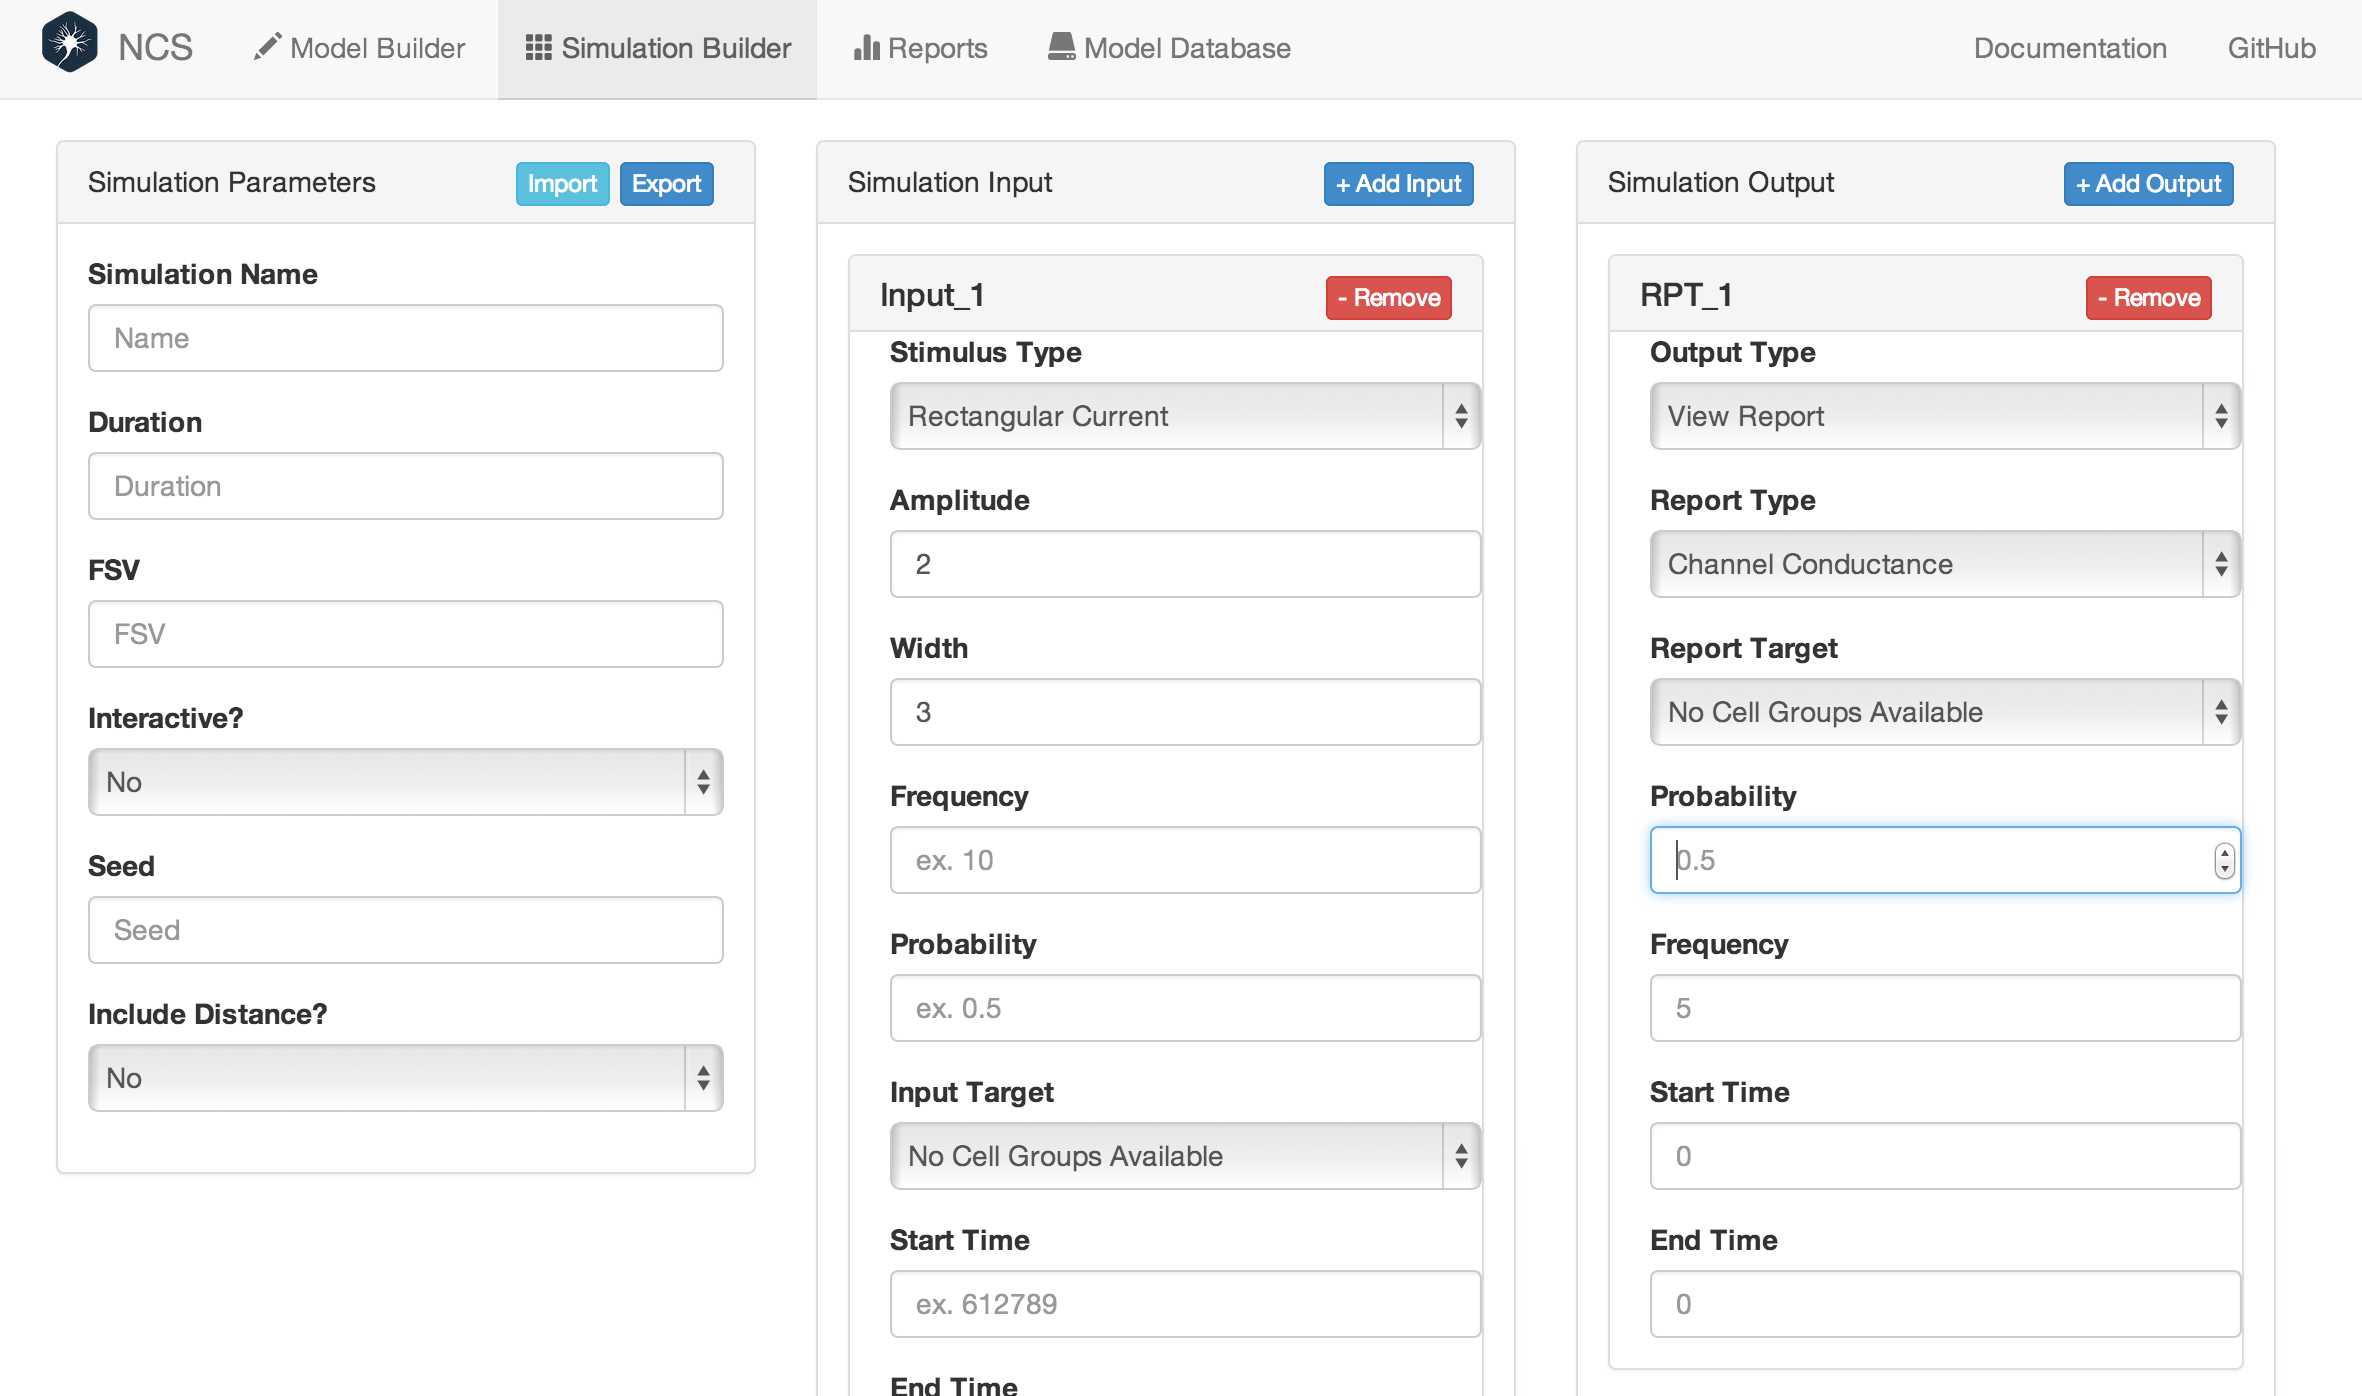
\includegraphics[height=\textheight,width=5in,keepaspectratio]{figures/sim_builder.png}
\caption[Sim Builder]{The sim builder provides the functionality for adding reports and stimuli to the simulation. The leftmost panel changes global simulation parameters, the middle panel controls stimuli, and the rightmost panel controls reports.\label{fig:sim_builder}}
\end{center}
\end{figure}

To view the results of a simulation, the user navigates to the report tab which is shown in Figure \ref{fig:reports}. The reports tab has the ability to view graphs of simulation data. This data can come from either a static report after the simulation has finished, or be streamed from NCS-Daemon and the simulator to the browser via a WebSocket interface. This feature gives researchers the ability to view simulation data in real-time. Graphs can be built from the data and exported to an SVG (vector) format for inclusion in high quality publications and posters. An example of one of these graphs is shown in Figure \ref{fig:report_graph}.

\begin{figure}
\begin{center}
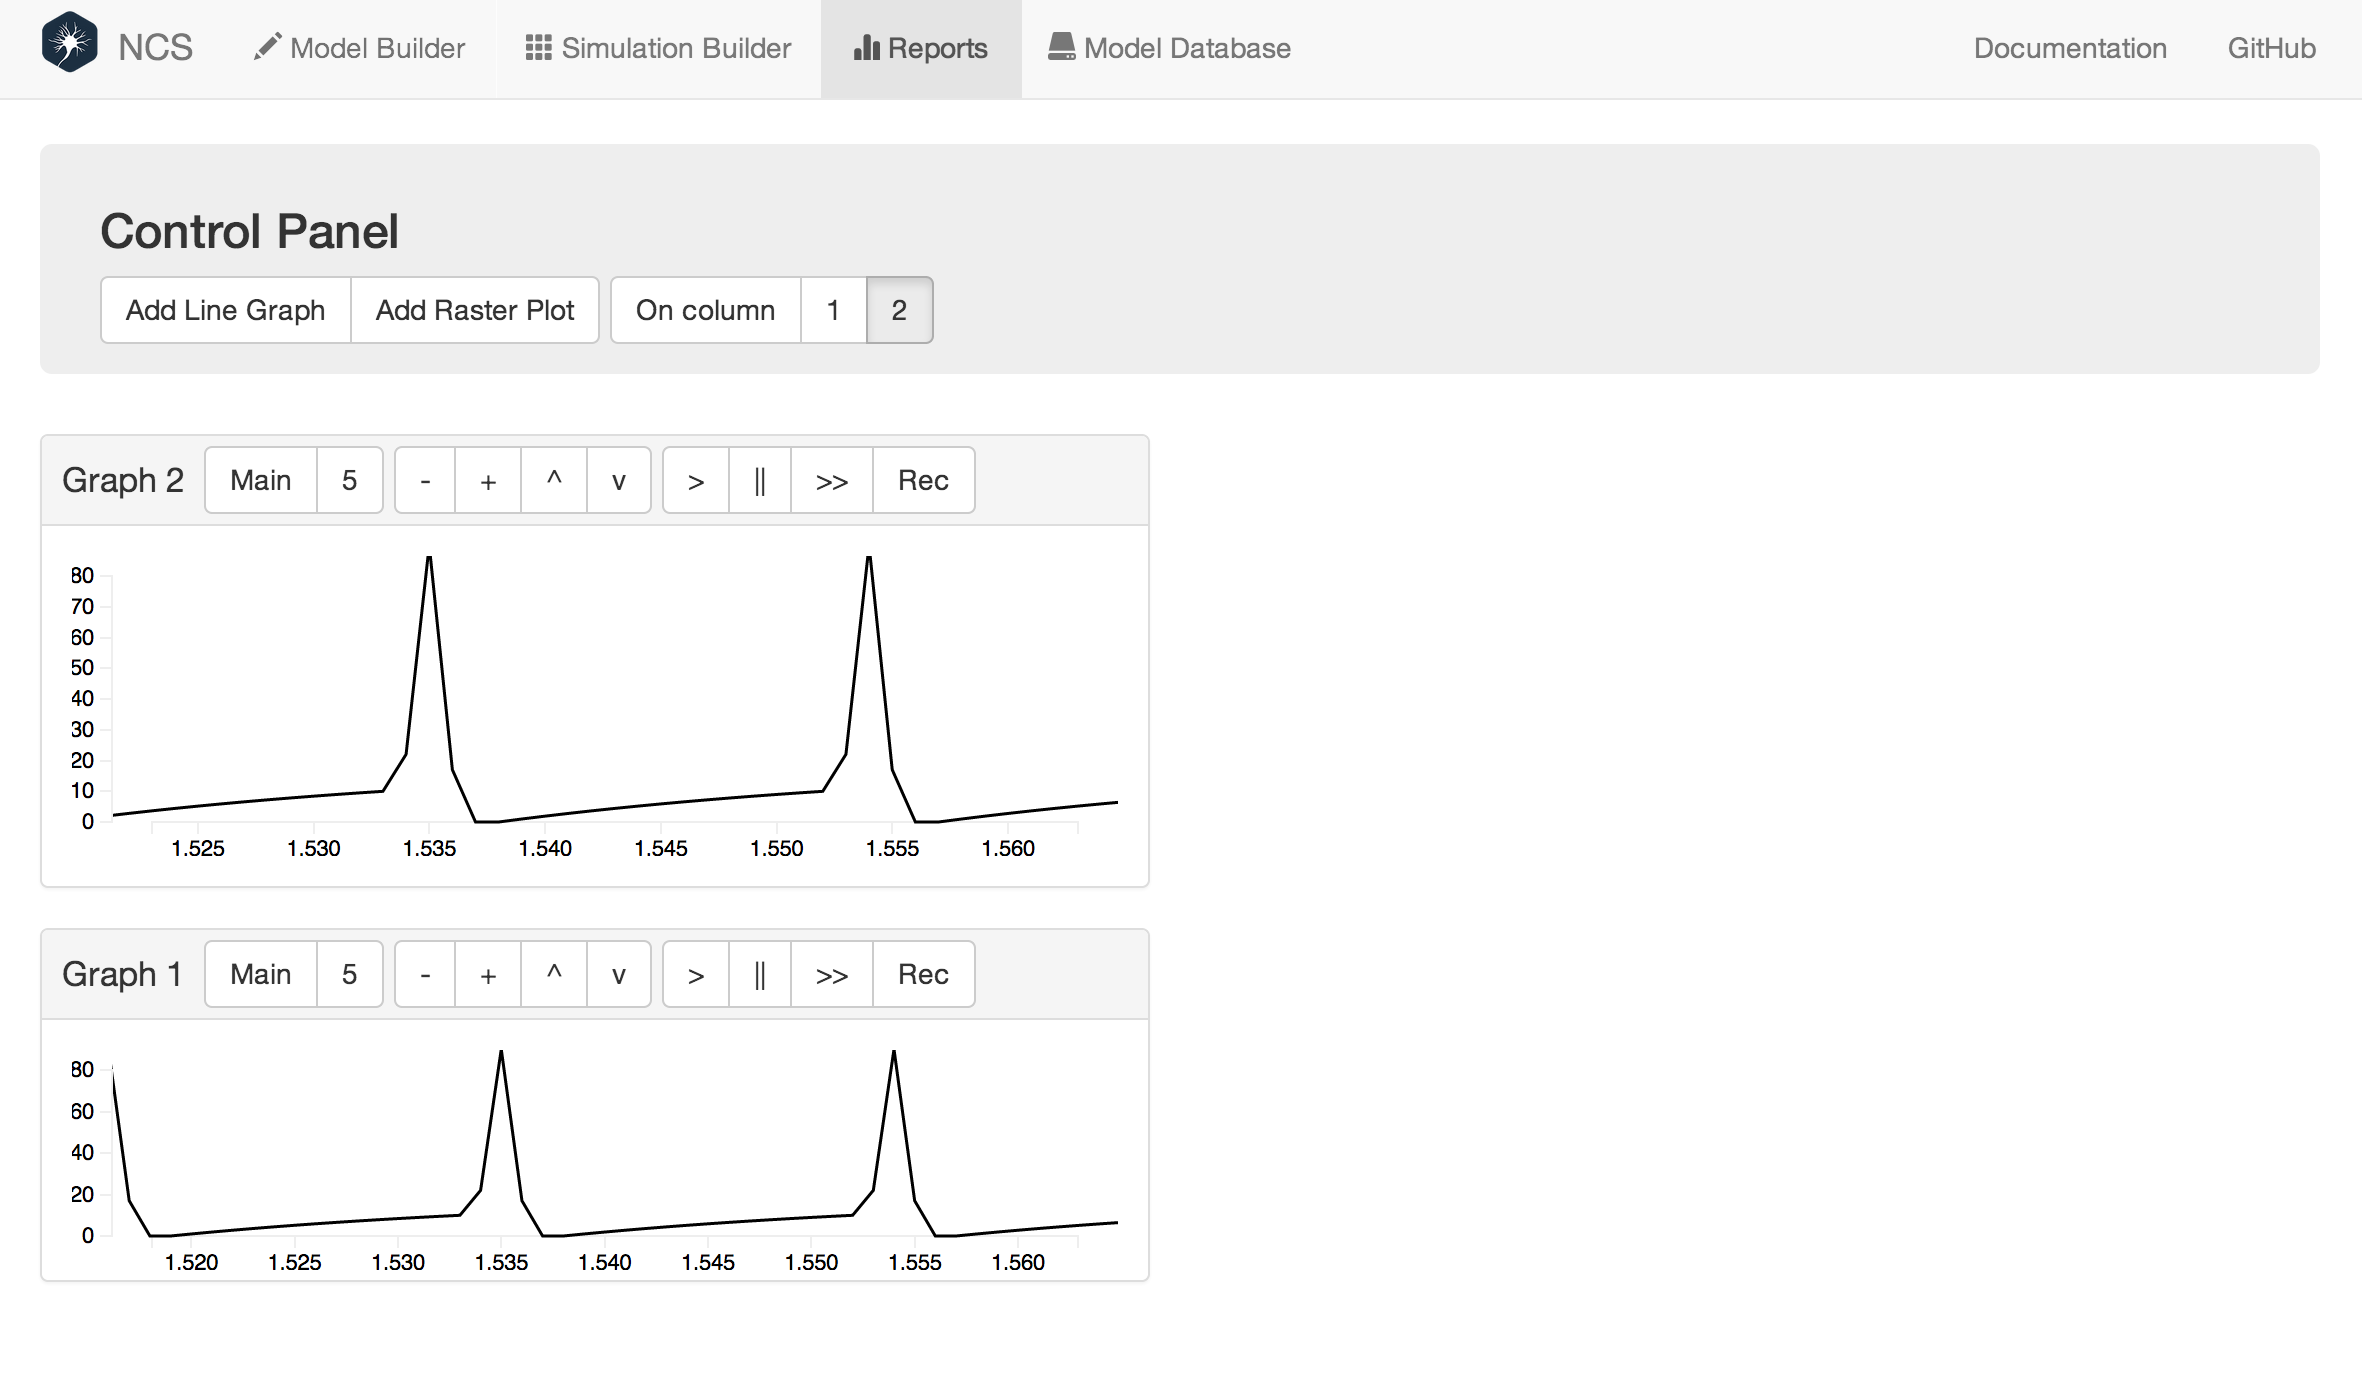
\includegraphics[height=\textheight,width=5in,keepaspectratio]{figures/reports.png}
\caption[Reports]{The reports tab allows users to view static and realtime data about a simulation. The graphs can be saved as high-quality SVG images for presentations or reports.\label{fig:reports}}
\end{center}
\end{figure}

\begin{figure}
\begin{center}
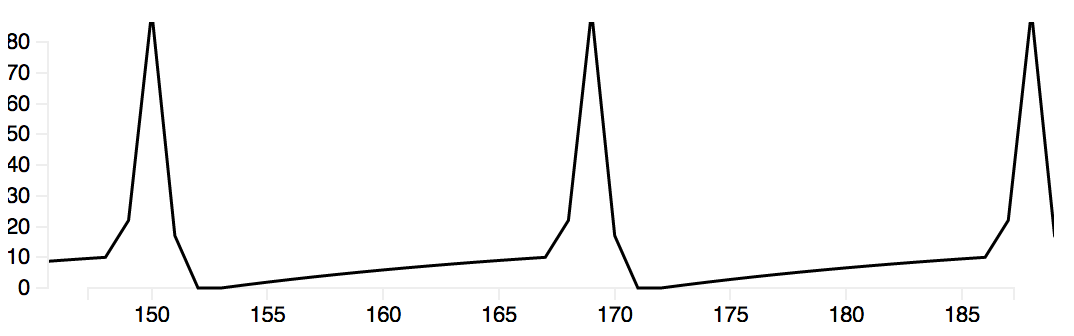
\includegraphics[height=\textheight,width=5in,keepaspectratio]{figures/report_graph.png}
\caption[Report Graph]{The reports generated in the reports tab can be exported as high-quality images for use in publications or in presentations.\label{fig:report_graph}}
\end{center}
\end{figure}

The robot simulation tab is still heavily in development. It allows simulation output to control the actions of a virtual robot in a 3D world and allow the observations of the robot on its environment to become inputs to the simulator. The simulator could be used to demonstrate the decision making ability of a brain model with the actions of the robot in the virtual environment, such as navigating a maze or performing actions when recognizing colors or patterns.








  \chapter{NCS}
\label{chapter:ncs}

\section{Introduction}

Introduce computational neuroscience

\section{Background}

\subsection{General Structure of the Brain}

\subsection{Simulation of Brain Structures}

\subsubsection{Single Neuron Simulations}

\subsubsection{Large-Scale Neural Simulations}

\subsection{Related Work}

Our Frontiers paper~\cite{frontiers_ncs}

\cite{multi_gpu_izh} paper with Corey on the multi Izh simulator

\cite{neuron_messages} Corey's paper on message passing 


\section{Design}

\subsection{Goals}

NCS6 was designed with three qualities in mind: extensibility, efficiency,
and approachability.  The first, extensibility, is a requirement in
order to enable mixed modeling, where parts of the simulation could be
computed one way while other parts are computed another. Enabling this
capability would allow more expensive precise computations to be done
in regions of interest while other regions could be approximated with
simpler computations. Additionally, it would allow different submodels
created using different components to be combined without the need to
convert the computational models used in one submodel to the computational
models used in another.

The second quality, efficiency, simply stems from a desire to maximize
resource utilization and minimize communication in order to maximize
throughput. By maximizing resource utilization, we seek to use
all available computational devices, not only the CPUs alone or the
GPUs alone but rather all device types working in tandem. We minimize
communication in hopes of ameliorating the necessity of a high-performance
network connecting compute nodes. Though efficiency can be at odds with
extensibility, we arrange our data structures in such a manner as to
minimize the loss of the former while gaining the boons of the latter.

Approachability deals with providing an effective user experience. That
is, running the simulator should be a simple task of executing the
simulator program, perhaps with a few input arguments. Furthermore,
the modeling aspect should be streamlined in a way such that repetitive
tasks are reduced without sacrificing the desired expressions of the user.

\subsection{Simulation Composition}

At its core, every simulation is composed of four elementary parts:
neurons, synapses, inputs, and reports. Neurons and synapses in this
scope are not exact analogs to their biological counterparts. Neurons
are the cell bodies that receive input currents and clamp voltages and,
under some defined circumstance, fires, transmitting spike signals
along its synapses. Synapses represent unidirectional connections from
one neuron to another. When the presynaptic neuron fires, the synapse
injects current into the postsynaptic neuron after some specified
delay. Inputs represent external stimuli that affect neurons. These
can have the effect of either augmenting the amount of current received
by a neuron or clamping the voltage of the neuron body to some precise
value. The final element, reports, specify the output component of the
system. Reports take either a collection of neurons or a collection of
synapses and output some desired value to some type of data sink.

The descriptions of the aformentioned elements were intentionally left
vague. In reality, the behavior of each element is governed by a selected
computational model, though some constraints are enforced. For example,
one neuron could be simulated following an Izhikevich model while another
could be simulated using an integrate-and-fire model. While the internal
behavior of the two cell types can diverge, both are still required
to provide two bits of information at each time step: whether the cell
fired and the cell voltage. They are both also provided with the same
set of input data: stimuli, total synaptic current, and the previous
neuron voltage value.

\subsection{Simulation Environment and Distribution}

The initial targeted computing environment for NCS6 was any, potentially
heterogeneous, cluster of one or more computers composed of some mix of
CPUs and CUDA-capable GPUs. Due to the way NCS is designed, expansion
to OpenCL devices would only require the implementation of certain stub
functions. Since all computing devices can potentially have different
performance characteristics, we first assign a relative computational
power rating to each device. The current method for estimating these
values is to multiple each device's clock speed by its number of compute
cores.

Given the relative power of each device, we distribute simulation
elements across them. The rationale behind our distribution method can
be traced back to the expected behavior of synapses. When a presynaptic
neuron fires, a synapse will, after some delay, inject current into the
postsynaptic neuron purely based on the state of the synapse itself
and the voltage of the postsynaptic neuron. As such, every synapse
is distributed with its corresponding postsynaptic neuron in order to
minimize the amount of data that must be passed between devices. With
such a scheme, the only data that must be passed across the cluster
during simulation is the firing state of every neuron. This state is a
boolean true/false value; thus, a single neuron's firing state can be
represented by a single bit. Inputs are similarly distributed. Since
each input can only affect a single neuron, inputs are distributed on
the same device as its associated neuron.

As for the distribution method itself, we first estimate the computational
cost of a neuron and all of its associated synapses and inputs. Since the
number of synapses generally greatly outnumbers the number of synapses by
several orders of magnitude, we use the number of synapses that affect
a given neuron as the neuron's computational cost. Neurons are  sorted
in order of decreasing cost and then distributed across all devices
in the cluster such that the device with the lowest load (total cost /
device power) receives the next neuron. Once all neurons are distributed,
their associated synapses and inputs are placed on the same devices. All
compute elements on each device are then reordered so that elements of
the same subtype (Izhikevich, LIF, etc.)  form contiguous blocks that
can later be consumed by plugins.

\subsection{Data Scopes and Structures}

Due to the distributed nature of NCS6, elements may be referenced in a
number of scopes that mirror the environment's hierarchy: plugin, device,
machine, and global (cluster). After the distribution is finished, every
element is assigned a zero-based ID for each scope. IDs are padded between
plugins so that data words for structures allocated in other scopes are
related to only one plugin. In general, this means that IDs are padded
to a factor of 32 (the number of bits in a word) between plugins. It is
important to note that IDs are only unique within the same element type;
that is, there can be both a neuron and a synapse with a global ID of 0.

Depending on which elements need access to other elements, certain
key data structures are allocated and accessed using different
scopes. Data that is specific to an element subtype is stored at the
plugin scope. Because synapses may need to access the membrane voltage
from their postsynaptic neurons in order to determine their synaptic
current contributions, membrane voltages are stored and accessed using
device level IDs. The reason is all postsynaptic neurons and their
associated synapses reside on the same device due to the way they are
distributed. However, because the spiking state of a synapse depends on
the spiking state of the presynaptic neuron, the spiking state of neurons
is accessed using a global level ID when updating synaptic spiking states.

\subsection{Simulation Flow}

The basic flow of a simulation is as follows: for each time-step, the
current from stimuli and synapses is computed and used to update the
state of every neuron. The resulting spiking state of each neuron is
then used to determine the spiking state of their associated synapses
in later time-steps.

To facilitate maximum utilization of computing devices, the simulation
is partitioned into several stages that can be executed in parallel as
long as the requisite data for a given stage is ready. Figure~\ref{fig:ncs_flow} 
illustrates this division of work (dark boxes) along with the required
data (light boxes) needed to simulate a particular stage and the data
that is produced once that stage has been updated. A publisher-subscriber
system is used to pass data buffers from one stage to the next. During
the simulation, a stage attempts to pull all necessary data buffers
from their associated publishing stages. The stage is blocked until
all the data is ready. Once it obtains all the required data buffers,
it advances the simulation by a single time-step and publishes its own
data buffer while releasing all the others that it no longer needs. When
all subscribers to a data buffer release it, the data buffer is added
back to its publisher's resource pool for reuse. For any given stage,
a limited number of publishable buffers are used to prevent a stage from
consuming all computational resources and getting unnecessarily ahead of
any other stages. For example, without limiting the buffer count, because
the input update stage requires no data from any other sources, the stage
could simulate all time-steps before a single neuron update is allowed
to occur, effectively adding a serial time cost to the overall run time.

\begin{figure}
\begin{center}
%\includegraphics[height=\textheight,width=\textwidth,keepaspectratio]{figures/ncs_simulation_flow.pdf}
\end{center}
\caption{Graph decomposition of an NCS simulation.}
\label{fig:ncs_flow}
\end{figure}

Within a single stage, further granularity is gained by parallelizing
across subtypes. As an example, if a device simulates both LIF Neurons
and Izhikevich Neurons, the plugins updating each can be executed
in parallel. Due to padding from the ID assignments, updates should
affect completely separate regions of memory, including operations
on bit vectors. Exceptions to this, such as when an input writes to
a device-indexed input current for its target neuron, are handled by
using atomic operations or by aggregating partial buffers generated by
each plugin. The method chosen depends on the type of device and its
memory characteristics. While plugins are allowed to update ahead of one
another, the results for from a stage at a given time-step will not be
published to subscribers until all plugins (in that stage) have updated
up to that time-step.

\subsubsection{Input Update}

The purpose of the input update stage is to compute the
total input current to each neuron on the device as well as any voltage
clamping that should be done. The input current is represented by an
array of floating point values, one for each neuron (including padding)
on the device, initialized to zero at the beginning of each time-step. The
voltage neurons are clamped and stored in a similar fashion where a bit
vector is used to select which neurons should actually be clamped.

Inputs are expected to be updated by input plugins designed to handle
their subtype. Other than the device-level Neuron ID for each Input that
is statically determined at the beginning of the simulation, input plugins
rely on no other data from any other stage of the simulation. As such,
they are allowed to simulate ahead of the rest of the system as long as
it has empty buffers that can be written to and published.

\subsubsection{Neuron Update}

Unlike the input update stage, the neuron update stage has two
dependencies: the input current per neuron published from the input update
stage and the synaptic current per neuron published by the synapse update
stage. Given these two pieces of information, this stage is expected to
produce the membrane voltage and spiking state of every neuron on the
device. Like the input current, the membrane voltage is represented by
an array of floating point values. On the other hand, the spiking state
is represented by a bit vector.

Similar to inputs, neurons are expected to be updated by neuron plugins
designed to handle their subtypes. Despite receiving and writing data out
into device-level structures, neuron plugins operate purely in plugin
space. This is possible due to the fact that each plugin is given a
contiguous set of device-level IDs during the distribution. As a result,
device-level data passed into each plugin is simply offset accordingly
to yield the appropriate plugin-level representation.

\subsubsection{Vector Exchange}

The result of the neuron update stage is the firing state
of every neuron residing on the device. However, synapses are distributed
purely based on the postsynaptic neurons and as such the presynaptic
neurons could possibly reside on a different device. Thus, to determine
synaptic spiking, the state of every neuron in the simulation must be
gathered first. Again, the publisher-subscriber scheme is used to pass
data asynchronously. However, rather than passing data between stages,
it is used to pass data between different data scopes.

Figure~\ref{fig:communication} shows the flow of the neuron spiking information
across a cluster. When the device-level vector exchanger receives a
local firing vector, the data is published to the machine-level vector
exchanger. Within this exchanger, the local vector is copied into a
global vector allocated in the system memory. Once all local device
vectors are copied for a single time-step, the complete machine-level
vector is broadcast to all the other machines in the cluster. After all
machines in the cluster finish broadcasting, the complete global firing
vector is published back to the device-level vector exchangers where it
is copied back into the appropriate type of device memory before being
published out to any subscribing stages.

\subsubsection{Firing Table Update}

With the firing state of every neuron in the
simulation, a device can determine when all of its synapses will receive
the firing based on a per-synapse delay value. Given the potential
range of delays, this information is stored within a synaptic firing
table. A row of the table is a bit vector representing the firing state
of every synapse on the device. The number of rows in the table depends
on the maximum delay of all local synapses. When this stage receives the
global neuron fire vector, each synapse checks its associated presynaptic
neuron for a firing state. If it is firing, the synapse adds its delay
to the current time-step to determine the appropriate vector which is
then modified by setting its bit to 1.

After updating the table for a single time-step, the table row associated
to that step can be published. However, up to N time-steps ahead of the
current time can be published, where N is the minimum delay across all
local synapses. This allows devices to simulate ahead of one another to
a point rather than being completely locked in step. Additionally, the
publication of these extra buffers at the beginning of the simulation
allows the data to start flowing through the simulation.

\subsubsection{Synapse Update}

Given the firing state of each synapse on the device,
the synapses themselves can be updated. Like the input update stage, the
synapse update stage produces the total synaptic current per device-level
neuron also represented by an array of floating point values. In terms
of operating spaces, synapse plugins update synapses that operate at
both the plugin and device levels, reading from the synaptic fire vector
while writing to the synaptic current vector.

\subsubsection{Reporting}

\subsection{Communication}
Intranode: between devices

Internode: between machines as an extension

\subsection{Reporting}
\subsection{pyNCS: Improving Quality of Life}

\cite{pynest} pyNEST

\section{Results}

\section{Conclusions}

  \chapter{caVR}
\label{chapter:cavr}

\section{Introduction}

\section{Background}

\subsection{Applications}

VFire~\cite{vfire}

RIST~\cite{rist}

Global Illumination~\cite{global_illumination}

\subsection{Hardware}

Output: Visual, Auditory, Haptic, Olfactory?

Input: Buttons, Analogs, DOFs

\subsection{Other Libraries}

FreeVR~\cite{freevr}

VRUI~\cite{vrui}

Hydra?

\section{Design}

\section{Results}

\section{Conclusions}

  \chapter{Conclusions and Future Work}
\label{chapter:conclusions}

\section{Conclusion}

To extend the NCS brain simulator, we have created a number of tools that allow users to interact with the simulator in a variety of ways. NCS-Daemon provides a base level of interaction, handling the lower-level operations on the simulator. It introduces a the client-server architecture to the ecosystem of neural simulators, allows for web-based interaction, organizes simulation data, and provides a way to stream real-time data from the simulation to clients. 

PyNCS creates a way for researchers to use the Python language to create models and interact with the simulator. The library provides features such as parameter checking that make it more user friendly and easier to debug than the minimalistic Python layer. This language binding also gives easy access to a number of scientific tools such as SciPy or NumPy that might be used to process the resulting data. 

Finally, the web interface provides a method to interact with the simulator without requiring any knowledge of programming. The interface allows users to build, run, analyze, and visualize neural simulations in a single web application. This tool, as well as PyNCS and NCS-Daemon, bring new technologies to the neural simulator landscape that has long been plagued with aging technologies, and allow researchers more effective ways of performing experiments and creating scientific breakthroughs.

\section{Future Work}

NCS and its surrounding tools provide a basic interface for working on brain simulations, but there is always more that could be done. Implementing a job queue for simulation queuing would be advantageous to waiting until another user is done to start a simulation. One could simply create the simulation and submit it and NCS-Daemon would run it when it reaches the front of the queue and notify the user in some way when the simulation is complete. 

Another possible addition would be an external robotics interface that would allow the simulator to interact with a ROS robot such as a PR2. By using ROS it would also allow a connection with a virtual robot in the ROS environment, or physical robot implementing the ROS software. With this ability, researchers could apply their models to real-world robotic scenarios.

A web-based realtime visualization of the simulation is currently being developed using WebGL that allows users to visualize the model they created while the simulation is running and see individual neurons firing\cite{cardozadesign}. The geometry would be streamed via a WebSocket dedicated to this purpose. The user can navigate around the model, change colors, and turn parts of the model on and off.

Interfaces can always be improved upon, and the NCS web interface is no different. As web technologies and interface design change and evolve, there will be a constant need to rework existing designs. The NCS web interface could use additional styling, better UI design, and additional features to make it more viable as a tool for building an simulating models, as well as analyzing the results.

Lastly, while Python was chosen to implement the client library for NCS (PyNCS), it is far from the only language option for interacting with the simulator. Since NCS-Daemon is implemented as a HTTP-based service, it can be easily expanded to other languages. Languages like Ruby would make an excellent candidate for another way to interact with the simulator.







  }


  %\nocite{*}  
  % bibliography
  {
	\newpage
  %\phantomsection\label{fdsjafklasjfdasjfjasfj}
	\baselineskip=13pt
    % \bibliographystyle{IEEEbib} % attempts to order based on appearance
	\addcontentsline{toc}{chapter}{Bibiliography}
	\bibliographystyle{plain} % attempts to order alphabetically by author
	\bibliography{bib}
  }
\end{document}
